% Copyright (C) 2014-2019 by Thomas Auzinger <thomas@auzinger.name>
%TZ: version slightly modified for ETIT thesis
 
\documentclass[draft,final]{vutinfth} % Remove option 'final' to obtain debug information.

% Load packages to allow in- and output of non-ASCII characters.
\usepackage{lmodern}        % Use an extension of the original Computer Modern font to minimize the use of bitmapped letters.
\usepackage[T1]{fontenc}    % Determines font encoding of the output. Font packages have to be included before this line.
\usepackage[utf8]{inputenc} % Determines encoding of the input. All input files have to use UTF8 encoding.

% Extended LaTeX functionality is enables by including packages with \usepackage{...}.
\usepackage{amsmath}    % Extended typesetting of mathematical expression.
\usepackage{amssymb}    % Provides a multitude of mathematical symbols.
\usepackage{mathtools}  % Further extensions of mathematical typesetting.
\usepackage{microtype}  % Small-scale typographic enhancements.
\usepackage[inline]{enumitem} % User control over the layout of lists (itemize, enumerate, description).
\usepackage{multirow}   % Allows table elements to span several rows.
\usepackage{booktabs}   % Improves the typesettings of tables.
\usepackage{subcaption} % Allows the use of subfigures and enables their referencing.
\usepackage[ruled,linesnumbered,algochapter]{algorithm2e} % Enables the writing of pseudo code.
\usepackage[usenames,dvipsnames,table]{xcolor} % Allows the definition and use of colors. This package has to be included before tikz.
\usepackage{nag}       % Issues warnings when best practices in writing LaTeX documents are violated.
\usepackage{todonotes} % Provides tooltip-like todo notes.
\usepackage{hyperref}  % Enables cross linking in the electronic document version. This package has to be included second to last.
\usepackage[acronym,toc]{glossaries} % Enables the generation of glossaries and lists fo acronyms. This package has to be included last.

% ADDED
%grey boxes for self citation
\usepackage{ntheorem}   % for theorem-like environments
\usepackage{mdframed}   % for framing
\theoremstyle{break}
\theoremheaderfont{\bfseries}
\newmdtheoremenv[
linecolor=gray!20,
leftmargin=00,
rightmargin=00,
backgroundcolor=gray!20,
innertopmargin=5pt,
ntheorem
]{Prev.Publ}{\textbf{Notice of adoption from previous publications in section}}{}
% allow full length citation of sources inside text
\usepackage{bibentry}
\usepackage{natbib}
\nobibliography*

% stop ADDED
\newacronym[plural=IDSs,firstplural=Intrusion Detection Systems (IDS)]{ids}{IDS}{Intrusion Detection System}
\newacronym{ml}{ML}{Machine Learning}
\newacronym[plural=NNs,firstplural=Neural Networks (NNs)]{nn}{NN}{Neural Network}
\newacronym[plural=ANNs,firstplural=Artificial Neural Networks (ANNs)]{ann}{ANN}{Artificial Neural Network}
\newacronym[plural=RNNs,firstplural=Recurrent Neural Networks (RNNs)]{rnn}{RNN}{Recurrent Neural Network}
\newacronym[plural=CNNs,firstplural=Convolutional Neural Networks (CNNs)]{cnn}{CNN}{Convolutional Neural Network}
\newacronym{bert}{BERT}{Bidirectional Encoder Representations from Transformers}
\newacronym{nlp}{NLP}{Natural Language Processing}
\newacronym[plural=GPUs,firstplural=Graphics Processing Units (GPU)]{gpu}{GPU}{Graphics Processing Unit}
\newacronym{lstm}{LSTM}{Long Short-Term Memory}
\newacronym{dlstm}{DLSTM}{Deep Long Short-Term Memory}
\newacronym{lstmsae}{LSTM-SAE}{LSTM-based Stacked Auto-Encoder}
\newacronym{lstmae}{LSTM-AE}{LSTM-based Auto-Encoder}
\newacronym{nids}{NIDS}{Network Intrusion Detection System}
\newacronym{iat}{IAT}{Interarrival Time}
\newacronym{bce}{BCE}{Binary Cross Entropy}
\newacronym{sgd}{SGD}{Stochastic Gradient Descent}
\newacronym{mae}{MAE}{Mean Absolute Error}
\newacronym{rmse}{RMSE}{Root Mean
Square Error}
\newacronym{smape}{SMAPE}{Symmetric Mean Absokute Percentage Error}
\newacronym{far}{FAR}{False Alarm Rate}
\newacronym{sel}{SEL}{Squared Error Loss}
\newacronym{relu}{ReLU}{Rectified Linear Unit}
\newacronym{mlm}{MLM}{Masked LM}
\newacronym{nsp}{NSP}{Next Sentence Prediction}
\newacronym{mts}{MTS}{Multivariat Time Series}


% Define convenience functions to use the author name and the thesis title in the PDF document properties.
\newcommand{\authorname}{Jonas Ferdigg} % The author name without titles.
\newcommand{\thesistitle}{Self-supervised Pre-training on LSTM and Transformer models for Network Intrusion Detection} % The title of the thesis. The English version should be used, if it exists.

% Set PDF document properties
\hypersetup{
    pdfpagelayout   = TwoPageRight,           % How the document is shown in PDF viewers (optional).
    linkbordercolor = {Melon},                % The color of the borders of boxes around crosslinks (optional).
    pdfauthor       = {\authorname},          % The author's name in the document properties (optional).
    pdftitle        = {\thesistitle},         % The document's title in the document properties (optional).
    pdfsubject      = {Subject},              % The document's subject in the document properties (optional).
    pdfkeywords     = {a, list, of, keywords} % The document's keywords in the document properties (optional).
}

\setpnumwidth{2.5em}        % Avoid overfull hboxes in the table of contents (see memoir manual).
\setsecnumdepth{subsection} % Enumerate subsections.

\nonzeroparskip             % Create space between paragraphs (optional).
\setlength{\parindent}{0pt} % Remove paragraph identation (optional).

\makeindex      % Use an optional index.
\makeglossaries % Use an optional glossary.
%\glstocfalse   % Remove the glossaries from the table of contents.

% Set persons with 4 arguments:
%  {title before name}{name}{title after name}{gender}
%  where both titles are optional (i.e. can be given as empty brackets {}).
\setauthor{}{\authorname}{BSc}{male}
\setadvisor{Univ. Prof. Dipl.-Ing. Dr.-Ing.}{Tanja Zseby}{}{female}

%\setauthor{Pretitle}{\authorname}{Posttitle}{female}
%\setadvisor{Pretitle}{Forename Surname}{Posttitle}{male}



% For bachelor and master theses:
\setfirstassistant{Univ.Ass. Dott.mag.}{Maximilian Bachl}{}{male}

% For dissertations:
\setfirstreviewer{Pretitle}{Forename Surname}{Posttitle}{male}
\setsecondreviewer{Pretitle}{Forename Surname}{Posttitle}{male}

% For dissertations at the PhD School and optionally for dissertations:
\setsecondadvisor{Pretitle}{Forename Surname}{Posttitle}{male} % Comment to remove.

% Required data.
\setregnumber{01226597}
\setdate{01}{01}{2001} % Set date with 3 arguments: {day}{month}{year}.
\settitle{\thesistitle}{Self-Supervised learning for Cyber Security Applications} % Sets English and German version of the title (both can be English or German). If your title contains commas, enclose it with additional curvy brackets (i.e., {{your title}}) or define it as a macro as done with \thesistitle.
%\setsubtitle{Optional Subtitle of the Thesis}{Optionaler Untertitel der Arbeit} % Sets English and German version of the subtitle (both can be English or German).

% Select the thesis type: bachelor / master / doctor / phd-school.
% Bachelor:
%\setthesis{bachelor}
%
% Master:
\setthesis{master}
\setmasterdegree{dipl.} % dipl. / rer.nat. / rer.soc.oec. / master
%
% Doctor:
%\setthesis{doctor}
%\setdoctordegree{rer.soc.oec.}% rer.nat. / techn. / rer.soc.oec.
%
% Doctor at the PhD School
%\setthesis{phd-school} % Deactivate non-English title pages (see below)

% For bachelor and master:
%\setcurriculum{Telecommunications} % Sets
\setcurriculum{Embedded Systems}{Embedded Systems} % Sets the English and German name of the curriculum.
%\setcurriculum{Media Informatics and Visual Computing}{Medieninformatik und Visual Computing} % 

% For dissertations at the PhD School:
\setfirstreviewerdata{Affiliation, Country}
\setsecondreviewerdata{Affiliation, Country}


\begin{document}

\frontmatter % Switches to roman numbering.
% The structure of the thesis has to conform to
%  http://www.informatik.tuwien.ac.at/dekanat

%\addtitlepage{naustrian} % German title page (not for dissertations at the PhD School).
\addtitlepage{english} % English title page.
\addstatementpage

%\begin{danksagung*}
%\todo{Ihr Text hier.}
%\end{danksagung*}

\begin{acknowledgements*}
\todo{Enter your text here.}
\end{acknowledgements*}

\begin{kurzfassung}
\todo{Ihr Text hier.}
\end{kurzfassung}

\begin{abstract}

\end{abstract}

% Select the language of the thesis, e.g., english or naustrian.
\selectlanguage{english}

% Add a table of contents (toc).
\tableofcontents % Starred version, i.e., \tableofcontents*, removes the self-entry.

% Switch to arabic numbering and start the enumeration of chapters in the table of content.
\mainmatter

%\input{intro.tex} % A short introduction to LaTeX.
%\input{chapter/}

\chapter{Introduction}

\section{Motivation} \label{sect.motivation}

With the progressing digitalization of evermore aspects of society, cyber security will always be a relevant issue as no system will ever be fully secure. Preventing possible cyber attacks by developing more robust systems is one way to mitigate the issue, the other is preventing already existing faults from being exploited as not every vulnerability can be patched easily as it is the case with e.g. DoS and bruteforce attacks. To stop such attacks it is necessary to identify them within the vast flow of ordinary network traffic which gives rise to the need of \glspl{ids}. State-of-the-art \glspl{ids} apply two methods to detect occurring attacks: Signature-based detection and statistical anomaly-based detection. Signature-based detection looks for known patterns or signatures within packets and data streams to identify incoming attacks. Statistical anomaly-based detection focuses on differentiating between normal and abnormal behavior in the system and raises an alert if the latter is identified. The problem with signature-based detection is that unknown attacks are ignored and anomaly-based detection is still not sufficiently accurate and prone to false positives. A machine learning based approach has the potential to combine both and overcome the downsides of each one has individually. As \gls{ml} is a rapidly developing field, its steady improvement fueled the advance of \gls{nn} based \glspl{ids} which start to show promising results \cite{fog_based_detection_survey_2020}, \cite{kitsune}, \cite{ml_ids_survey}. \glspl{nn} however are still mostly trained in a supervised fashion, namely by providing labeled examples of cyber attacks for the \gls{nn} to learn from. This poses the problem, that only known attacks can be identified, but new attacks that are sufficiently similar to old attacks can also be identified, which is not the case with mere signature-based detection. As with every form of supervised training on \glspl{nn}, labeled data is harder to come by while unlabeled data is often abundant and certainly so for network traffic data. For this reason, self-supervised training/pre-training is seeing increased use in the realm of \gls{ml}, as unlabeled data can be used to boost the performance without the need for expensive labeled data. One of the most noteworthy examples of the effectiveness of self-supervised pre-training for Neural Networks in the realm of \gls{nlp} is \gls{bert} \cite{bert} developed by Jacob Devlin \textit{et alteri} from Google AI Language. \gls{bert} is based on the state-of-the-art transformer architecture \cite{attention} and uses a series of proxy tasks like word masking and next sentence prediction to teach the network about syntax and grammar in a self-supervised fashion i.e. without using labeled data. The pre-trained network can then be fine-tuned for more specific tasks like question answering or text classification. Analogous, it would be highly beneficial if these or similar pre-training mechanisms could be used to bolster performance of \gls{ml} based \glspl{ids} by improving the classification of network flows, at the most basic level, into cyber attack vs. no cyber attack. \par
As the technologies mentioned above are fairly recent (Transformers Dec 2017, \gls{bert} May 2019) and the design space for solutions in the context of \gls{ml} for cyber security is substantial, there has not yet been sufficient inquiry into the possibilities of these new methods when applied to the problems posed by Intrusion Detection and cyber attack classification. \gls{nn} performance also improves with the steadily increasing capabilities of modern \glspl{gpu} which makes this a promising concept that can be improved upon by future more powerful hardware. 

%\subsection{Objective} \label{sect.objective} 
%TEXT

\section{Research Questions} \label{sect.research_questions}

In this thesis we inspect if the flow classification performance of \glspl{lstm} and Transformer-Encoder networks can be improved with self-supervised pre-training in a scenario where only little labeled and a lot of labeled data is available. In our experiments we are looking at scenarios where the ratio of labeled to unlabeled data is 1:8, 1:80 and 1: for labeled to unlabeled data. For performance we are mainly looking at the accuracy of classification, but we are also keeping track of the \gls{far}. The problem to solve is a binary classification problem for which the model is to group flows into \textit{attack} and \textit{no-attack}. 

\begin{itemize}
	\item R1: Can self-supervised pre-training improve the flow classification capabilities of an \gls{lstm} model?
	\item R2: Can self-supervised pre-training improve the flow classification capabilities of a Transformer-Encoder model?
	\item R3: Which pre-training tasks improve accuracy and which do not?
	\item R4: If improvement is possible, how can it be explained?
\end{itemize}


\section{Approach} \label{sect.approach}

To answer these questions we conduct a series of experiments. In these experiments we devised different proxy tasks for the model to solve in a self-supervised fashion. Solving these proxy tasks serves as pre-training for the network during which it learns the structure of the data and to form abstract representations within its latent space. After the pre-training we train the network with very little labeled training data to teach it how it should classify the flows. These experiments show if pre-training can improve accuracy of the model when compared to only training it with the same amount of labeled data but no pre-training. They also show which pre-training methods are more and which are less beneficial for classification accuracy.

\section{Contribution} \label{sect.contribution}

\begin{itemize}
	\item Implementation of a pre-trainable \gls{lstm} model and training suite
	\item Implementation of a pre-trainable Transformer-Encoder model and training suite
	\item Inquiry into the benefits of pre-training for sequence-to-sequence models in the context of \glspl{nids}
	\item Development of new pre-training methods for \glspl{lstm} and TransformerEncoder models in the context of \glspl{nids}
\end{itemize}

Here provide a list of the contributions of your work.

Suggestion (especially for dissertations): provide a table with research questions, methods used to answer each, and major findings and the section in which to find details.

\section{Structure} \label{sect.structure}

After this introduction section we will provide some background information and define terminology used throughout the thesis \ref{sec:background}. Subsequently we provide an overview of the current state-of-the-art of \glspl{nn} for sequence-to-sequence modeling \ref{sec.state_of_art}, pre-training for such models and \gls{ml} supported \glspl{nids} in general. Reasoning behind our methodology, and other decisions made, can be found in its dedicated section \ref{sec:methodology}. A detailed description of the conducted experiments can 
be found in the section \textit{Experiments} \ref{sec:experiments} with the goal to make them as reproducible as possible. A structured comprehension of experiments conducted is provided in the section \textit{Results} \ref{sec:results}. Finally, in the sections \textit{Discussion} \ref{sec:discussion} and \textit{Conclusion} \ref{sec:conclusion} we discuss successes and failures and draw conclusions from our findings, including pointers for future research. 


\newpage
\chapter{Background} \label{sec:background}

\glspl{ann} have shown great improvements over the last years due to increasing compute power, more sophisticated models and smarter training algorithms \todo{cite papers}. \gls{ml} and \glspl{ann} have long found their way into many commercial applications and many scientific fields have successfully applied this relatively new method of data processing to further their own research. \todo{cite papers} It was only logical that researchers and companies have also started to look into the possible benefits this emerging technology could have for Network Security applications \todo{cite papers}. \glspl{ann} are especially suited for \glspl{ids} due to their capability to classify data with high accuracy. To harness the power of \gls{ml} for the purpose of Network Security, we made use of existing methods and models which we will summarize in this section.

\subsection{Machine Learning} \label{sec:background:ml}

\subsection{Artificial Neural Networks} \label{sec:background:ann}

Named after their resemblance to neurons in a brain, \glspl{ann} are systems comprised of connected nodes called \textit{artificial neurons}. Analogous to synapses, nodes communicate \textit{via} connections called \textit{edges} by sending "signals" to other nodes. Signals are represented as scalar real numbers. The output signal from a sending node is multiplied by the weight of the edge the signal is "traveling" on. Each node calculates its output signal by applying a non-linear function to the sum of its input signals. Signals travel forward through the network from the first to the last layer, but usually not within layers. There are various types of \glspl{ann} like \glspl{rnn} or \glspl{cnn} which have many derivations themselves but they all operate on the before stated principal of signals traveling through the network which get transformed at each node by a differentiable non-linear function. The most popular non-linear function at this time is the \gls{relu} function. Without training an \gls{ann} performs an input transformation that depends on the initialization values of its weights, often called \textit{parameters}. The network is trained to perform a desired transformation by adjusting its weights/parameters through virtue of \textit{back-propagation}. The network produces output $\hat{y}$ at the last layer after processing input $x$. A scalar cost/loss value is calculated by a \textit{loss function} $C(\hat{y}, y)$ as a measure of difference between the networks output $\hat{y}$ and the target output $y$. For classification tasks the loss function is usually cross entropy loss \todo{reference cross entropy loss} and for regression \gls{sel} is typically used. Back-propagation computes the gradient of every weight in the network with respect to the loss function by applying the chain-rule for every layer down to every weight. After calculating the gradient for every weight, a gradient method like \gls{sgd} is used to iteratively update all weights in order to minimize $C(\hat{y}, y)$. \todo{find/create graphic}

\subsection{Recurrent Neural Networks} \label{sec:background:rnn}

The broader concept behind all \glspl{rnn} is a cyclic connection which enables the \gls{rnn} to update its state based on past states and current input data \cite{rnn_review}. Typically, an \gls{rnn} consists of standard tanh nodes with corresponding weights. There are different kinds of \glspl{rnn} like continuous-time and discrete-time or finite impulse and infinite impulse \glspl{rnn}. Here we will only look at discrete-time, finite impulse \glspl{rnn} as we will only be using those. This type of network, e.g. the Elman network \cite{rnn_elman}, is capable of processing sequences of variable length by compressing the information from the whole sequence into the \textit{hidden layer}. \todo{give a more formal description of RNNs} The model produces one output token for each input token, so the transformation is sequence-to-sequence where input and output sequences are of equal length. One input sequence consists of a sequence of real valued vectors $x^{(t)} = x^{(1)}, x^{(2)}, ... , x^{(T)}$ where $T$ is the sequence length. From this input sequence, an output sequence of real valued vectors $\hat{y}^{(t)} = \hat{y}^{(1)}, \hat{y}^{(2)}, ... , \hat{y}^{(T)}$ is produced. To train an \gls{rnn} 
pairs of input and target sequences $(x^{(t)}, y^{(t)})$ are provided from which, analogous to the training of \glspl{ann} in general\ref{sec:background:ann}, a differentiable loss function $C(\hat{y}^{(t)}, y^{(t)})$ can be calculated which can again be minimized by applying back-propagation. In theory, \glspl{rnn} can process data sequences of arbitrary length, but the longer the sequence, the deeper the network gets i.e. the longer the gradient paths. This leads to complications when relevant tokens are further apart in the sequence as the \gls{rnn} is not capable of handling such "long-term dependencies" \cite{rnn_review}. Long gradient paths in \glspl{rnn} might also cause the gradient to become either very small or very large, which results in the known \textit{vanishing gradient} or \textit{exploding gradient} problems correspondingly and cause training to either stagnate or diverge. The \gls{lstm} improves upon \glspl{rnn} by making the gradient more stable and allowing long-term dependencies to be considered in the learning process.
\todo{find/create graphic}

\subsection{Long Short-Term Memory}

Introduced by Hochreiter and Schmidhuber in 1997 \cite{lstm_origin}, the \gls{lstm} model mitigates the vanishing and exploding gradient problem by replacing the tanh nodes in the hidden layer of a conventional \gls{rnn} with \textit{memory cells} as seen in \ref{fig:background:lstm}. 
A memory cell is comprised of \textit{input node}, \textit{input gate}, \textit{internal state}, \textit{forget gate} and \textit{output gate}. 

\begin{figure}[h]
	\centering
	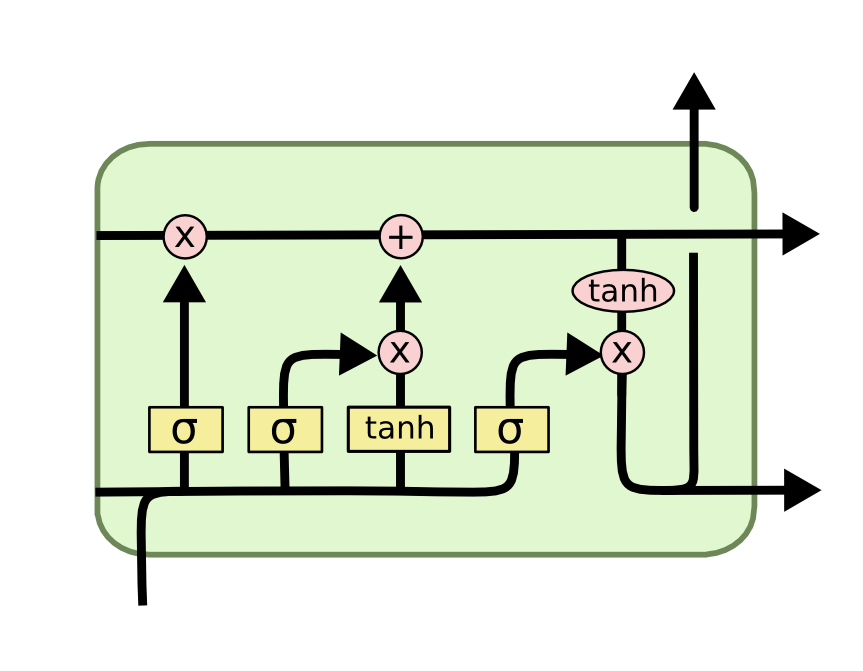
\includegraphics[width=1\textwidth]{img/lstm2.png}
	\caption{One \gls{lstm} memory cell \cite{rnn_zachary}}
	\label{fig:background:lstm}
\end{figure}
In contrast to an ordinary \gls{rnn}, an \gls{lstm} has two memory states: the hidden state $h^{(t)}$ and the \textit{cell state} $C^{(t)}$. Three gates enable the cell to control the flow of information and its effects on the cell state. For this purpose, gates in an \gls{lstm} consist of a point-wise multiplication with a vector that holds values between 0 and 1. The three sigma activations seen in \ref{fig:background:lstm} produce the gate vectors. The input gate $i^{(t)} = \sigma(W^i[h^{(t-1)},x^{(t)}] + b^i)$ controls whether the memory cell is updated. The forget gate $f^{(t)} = \sigma(W^f[h^{(t-1)},x^{(t)}] + b^f)$ controls how much of the old state is to be forgotten. The output gate $o^{(t)} = \sigma(W^o[h^{(t-1)},x^{(t)}] + b^o)$ controls whether the current cell state is made visible. The weight matrices $W^i, W^j$ and $W^o$ decide how information is processed by the cell and are learned parameters. The cell state is updated by addition with the vector $\bar{C}=\tanh(W^C[h^{(t-1)},x^{t}]+b^C)$ after multiplication with the input gate vector $i^{(t)}$. The repeated addition of a $\tanh$ activation distributes gradients and vanishing/exploding gradients are mitigated.

\subsection{Adam Optimizer}

\subsection{Attention and Transformers}

2017 Vaswani et al. published a paper with the ominous title "Attention is All you Need" \cite{attention_origin}, referring to the already known attention mechanism which is used to model dependencies within a data sequence over longer distances. The authors proposed the Transformer model consisting entirely of self attention mechanisms to model sequences and therefore diverge from the recurrent architectures of \glspl{rnn} and \glspl{lstm}. Attention is a mechanism to capture contextual relations between tokens in a sequence, e.g. words in a sentence. For every token in the input sequence, an attention vector is generated which represents how relevant other tokens in the input sequence are to the token in question. While attention can be implemented in different ways, the authors chose the scaled dot-product attention defined as 

\begin{equation}
	Attention(Q,K,V) = softmax(\frac{QK^T}{\sqrt{d_k}})V
\end{equation}

\begin{figure}[h]
	\centering
	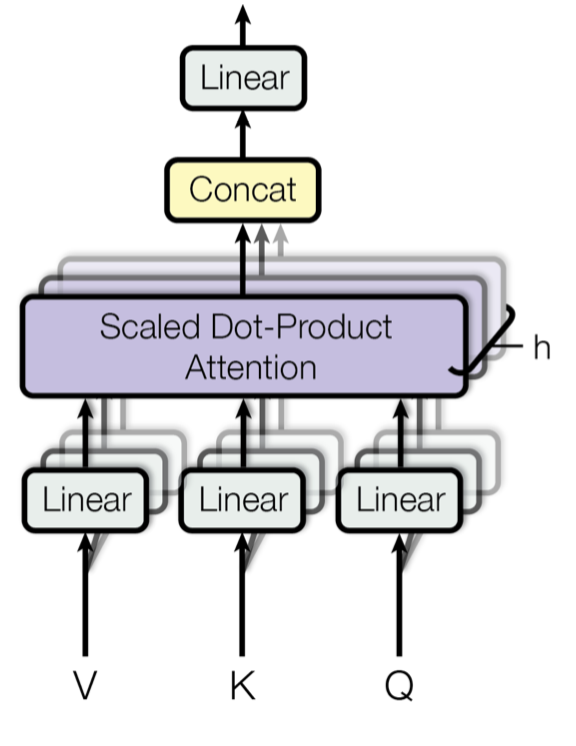
\includegraphics[width=0.3\textwidth]{img/attention.png}
	\caption{Self attention layer of Transformer by \cite{attention_origin}}
	\label{fig:attention}
\end{figure}

"An attention function can be described as mapping a query and a set of key-value pairs to an output" \cite{attention_origin}. $Q$, $K$ and $V$ are matrices composed of query, key and value vectors for every token with respect to every other token in the sequence.
Vaswani et al. proposed the use of Multi-Head Attention mechanism suggesting the use of multiple independent attention heads which are generated by linear projection of the original $Q, K$ and $V$ matrices by different learned matrices $W^Q_i, W^K_i$ and $W^V_i$ for $i = 1, ... ,h$ where $h$ is the number of desired attention heads. The attention vectors of the different attention heads are again concatenated and projected by matrix $W^Z$ again resulting in a single combined attention vector instead of $h$ vectors. This results in the formulation 

\begin{equation}
	head_i = Attention(QW^Q_i, KW^K_i, VW^V_i), i = 1, ..., h
\end{equation}

\begin{equation}
	MultiHead(Q,K,V) = Concat(head_1, ..., head_h)W^O
\end{equation}

depicted in figure \ref{fig:attention}. The Multi-Head Attention block from \ref{fig:attention} is
used in the Transformer encoder block \ref{fig:transformer_encoder} together with a fully-connected feed forward network. After each sub-layer (Multi-Head Attention, Feed Forward) layer normalization is applied and a residual connection originating from the input to the sub-layer is added as can again be seen in figure \ref{fig:transformer_encoder}. The output of each sub-layer is hence defined as $LayerNorm(x + Sublayer(x))$ where $Sublayer$ is either a Feed Forward or a Multi-Head Attention function. While there is more to the Transformer model, for our experiments we are only using the parts described here.


\begin{figure}[h]
	\centering
	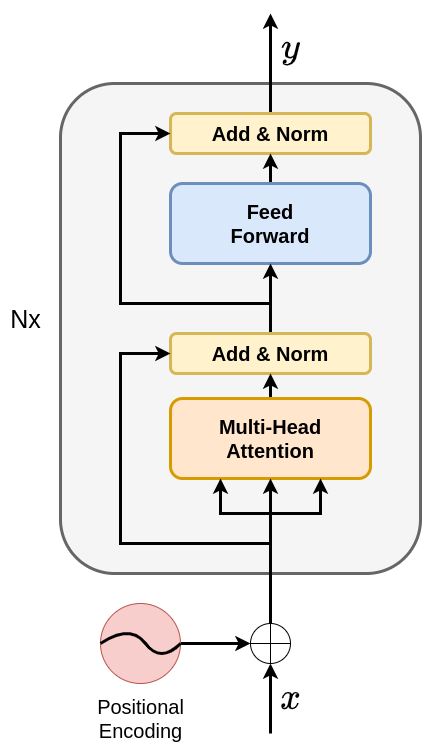
\includegraphics[width=0.4\textwidth]{img/transformer_encoder.png}
	\caption{Transformer Encoder Model as proposed by \cite{attention_origin}}
	\label{fig:transformer_encoder}
\end{figure}

\subsection{Self-supervised Learning}

\subsection{Auto Encoder} \label{subsec.autoencoder}

\subsection{Pre-Training and Fine Tuning}

\subsection{Terminology} \label{subsec.terminology}

In addition: Abbreviations and mathematical notation should be put in a list in the beginning of the thesis 

\newpage
\chapter{State of the art} \label{sec:stateofart}

As the topic of this thesis is rather specific, comparable research is hard to find. Overall, the thesis works on the two subjects of unsupervised pre-training for \glspl{nn} and for \gls{ml} supported \gls{nids}. Here we are looking at state-of-the-art research of both aspects individually.

\section{Self-supervised Pre-training for LSTMs and Transformer Networks}

When it comes to machine learning, rapid progress has been made over the past years. Frameworks such as PyTorch \cite{pytorch} and Tensorflow \cite{tensorflow} have made the technology accessible to people without a background in computer science. More than 11 thousand papers in the category "Computer Science - Artificial Intelligence (cs.AI)" have been published on arXiv.org \cite{arxiv} within only the last year. With steadily increasing processing capabilities, vast amounts of data can be used to train ever growing \glspl{nn} within an acceptable timeframe. E.g. the largest variant of Google's \gls{bert} algorithm has 340 million parameters and was trained on a dataset of 3.3 Billion words \cite{bert}. \par

\subsection{BERT: Pre-training of Deep Bidirectional Transformers for Language Understanding}

Google's BERT \cite{bert} by Jacob Devlin et al. effectively uses a Deep Bidirectional Transformer model, often referred to as Transformer Encoder, for various \gls{nlp} tasks, both on sentence and word level, like question answering, natural language inference, sentiment analysis, paraphrasing and others. At the time it was published, it produced the highest recorded GLUE \cite{glue} score of 80.5\% advancing it by 7.7\% over the former top scorer. It uses the WordPiece \cite{wordpiece} embedding resulting in a 30,000 token vocabulary. It was pre-trained in a fully unsupervised fashion on all sentences in the English Wikipedia (2,5 Billion words) and the BooksCorpus \cite{books_corpus} containing 800 Million word. The pre-training consisted of two proxy tasks: \gls{nsp} and \gls{mlm}. For \gls{nsp}, two sections of text, A and B, separated by a [SEP] token are fed into the model at the same time. 50\% of the time, B is the next section that follows A in the original text. 50\% of the time it is a random sentence from the corpus. The model is tasked with predicting, if sentence B follows sentence A. For \gls{mlm}, 15\% of the input tokens are hidden from the model by replacing with a [MASK] tokens. The model is tasked with reconstructing the masked tokens. Both of those pre-training tasks are performed at the same time. The pre-trained model is then fine-tuned to perform a specific down-stream task. \par
This two stage approach, pre-training and fine-tuning, produces a reusable pre-trained model which can then be fine-tuned relatively swiftly (Jacob Devlin et al. state that it takes at most an hour of fine-tuning on a \gls{gpu} to replicate all results in the paper) to solve various \gls{nlp} tasks. For this thesis, we use the same approach to pre-train our models in an unsupervised fashion and then fine-tune them with a small amount of labeled data to teach them the down-stream task of classifying network flows. We also use the pre-training task of masking parts of the input data for the model to reconstruct for both our \gls{lstm} and Transformer networks. The \gls{nsp} task is not feasible in our situation, as network flows don't have an order other than the time of occurrence, and therefore flows don't have a semantically identifiable successor or predecessor.

\subsection{Unsupervised Learning of Video Representations using LSTMs} \label{sec:stateofart:unsupervised_video_lstm}

The use of unsupervised learning is not limited to Transformer networks. As early as 2016, before the rise of Transformers, Nitish Srivastava et al. showed in their paper "Unsupervised Learning of Video Representations using LSTMs" \cite{unsupervised_learning_lstms} that unsupervised learning on \glspl{lstm} can have a positive impact on subsequent classification tasks. The authors use video data to train their models in frame prediction and auto encoding as the proxy tasks with the goal of improving accuracy in human action recognition, based on evaluation with the UCF-101 and
HMDB-51 datasets. They experimented with two types of video representations: patches of image pixels and high-level representations ("percepts") of video frames extracted by a convolutional net. They used 13,320 videos with an average length of 6.2 seconds belonging to 101 different action categories. \par
The auto-encoding property of the model is achieved by concatenating two \glspl{lstm}, with one performing the function of encoder and one of decoder. The goal is to produce a sequence2sequence model capable of reconstructing the input sequence after being forced to compress the input data. The input sequence is first processed by the encoder \gls{lstm} to produce an output of constant length (in their case, the hidden size of the encoder \gls{lstm}). The resulting vector is then fed into the decoder which is tasked with reconstructing the input sequence in reverse order. Here, the decoder can be configured to either be \textit{conditioned} or \textit{unconditioned}. A conditioned decoder uses the output of the last \gls{lstm} stage as input for the next stage. An unconditioned decoder uses the corresponding input token (ground truth) as input for the next stage. The latter practice is also called \textit{teacher forcing}. \par
The second unsupervised task to train the \gls{lstm} consists of predicting multiple future video frames. For this, again two consecutive \gls{lstm} networks are used: an encoder and a predictor \gls{lstm}. The first network is fed the frame representation of part of a short video and again produces a fixed sized output vector to be used by the predictor \gls{lstm}. The second \gls{lstm} is then tasked with producing the remaining frames. Same as with the auto-encoder the predictor \gls{lstm} can either be conditioned or unconditioned. \par
The authors then proposed a composite model as can be seen in figure \ref{fig:stateofart:unsupervised_lstm_composite} where both proxy tasks, reconstructing the input and predicting the future, are combined to produce a single model.

\begin{figure}[h]
	\centering
	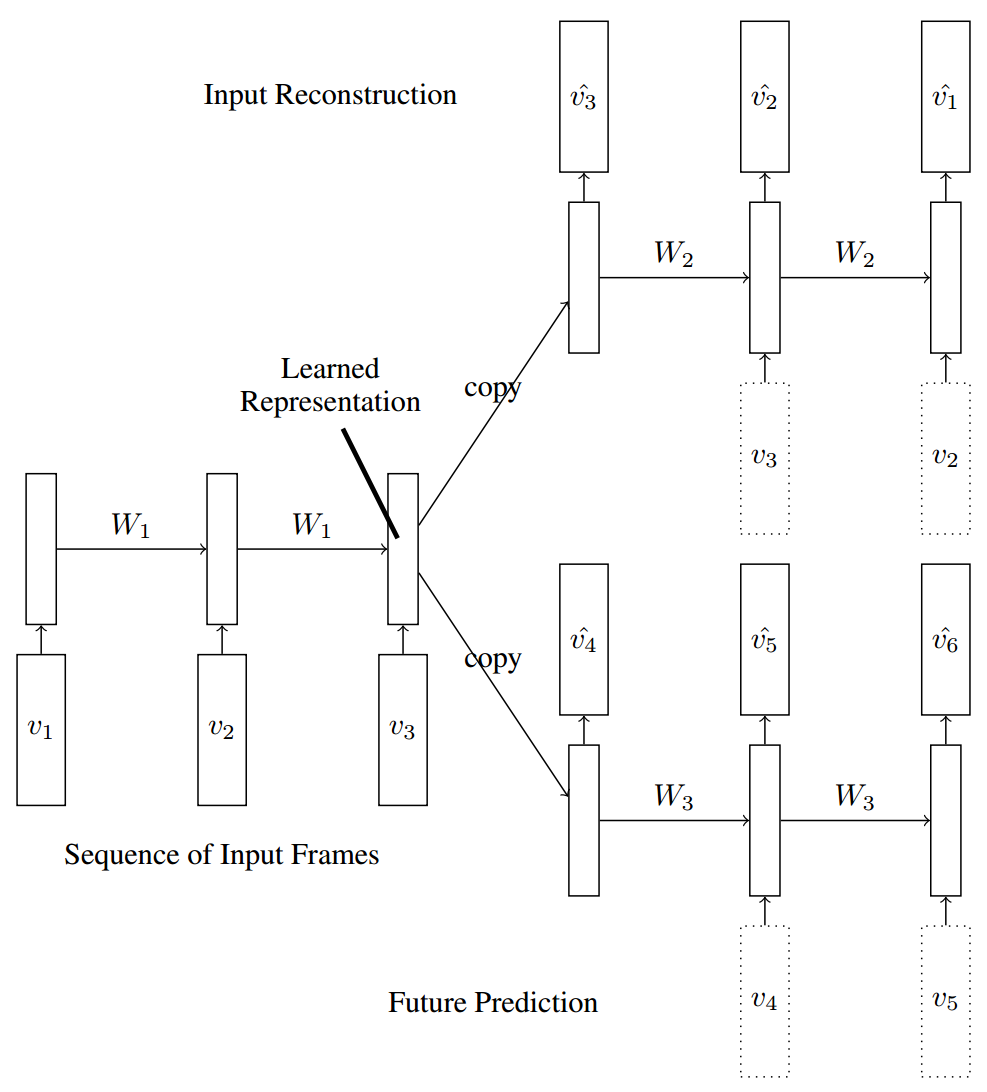
\includegraphics[width=0.7\textwidth]{img/unsupervised_learning_with_lstms_composite.png}
	\caption{Composite model for input reconstruction and future prediction \cite{unsupervised_learning_lstms}}
	\label{fig:stateofart:unsupervised_lstm_composite}
\end{figure}

The pre-trained models are then finetuned for their classification task on the mentioned training datasets.
With the pre-trained + finetuned composite model, the authors achieved an absolute increase of 1.3\% accuracy for both the UCF-101 and the HMDB-51 datasets over a conventional \gls{lstm} classifier as can be seen in table \ref{table:stateofart:unsupervised_learning_results}.

\begin{table}[]
	\begin{tabular}{l c c c}
		\thead{Model} & \thead{UCF-101 \\ RGB} & \thead{UCF-101
\\ 1-frame flow} & \thead{HMDB-51 \\
RGB} \\ \hline
		\midrule
		Single Frame & 72.2 & 72.2 & 40.1 \\
		\midrule
		LSTM classifier & 74.5 & 74.3 & 42.8 \\
		\midrule
		Composite LSTM
Model + Finetuning & 75.8 & 74.9 & 44.1 \\
	\end{tabular}
	\caption{Summary of results on Action Recognition \cite{unsupervised_learning_lstms}}
	\label{table:stateofart:unsupervised_learning_results}
\end{table}

For our thesis we used the same Auto-Encoder and composite model for pre-training as explained in sections \ref{sec:experiments:lstm_auto_encoder} and \ref{sec:experiments:lstm_composite}. We tried with both conditioned and unconditioned models, comparing results in section \ref{sec:results}.

\subsection{Unsupervised pre-training of
a Deep LSTM-based Stacked
Autoencoder for Multivariate time
Series forecasting problems} \label{sec:stateofart:unsupervised_learning_lstms_timeseries}

In their 2019 paper \cite{unsupervised_learning_lstms_timeseries} Alaa Sagheer et al. explore the benefits of unsupervised pre-training using stacked \gls{lstm} auto encoders with subsequent supervised finetuning. Their goal was to improve the prediction capabilities for \gls{mts} problems. In their previous paper \cite{dlstm_time_series_forecasting}, the authors showed the effectiveness of \gls{dlstm} based models for \gls{mts} prediction tasks. In their 2019 paper, they showed the improvements resulting from pre-training when compared to an initial random initialization of weights when working with \gls{dlstm} models. Compared to shallow \gls{lstm} networks, \gls{dlstm} networks contain multiple layers of \gls{lstm} cells stacked on each other. Information travels the network from left to right and from bottom to top as is depicted in figure \ref{fig:stateofart:unsupervised_learning_with_lstms_dlstm}. 

\begin{figure}[h]
	\centering
	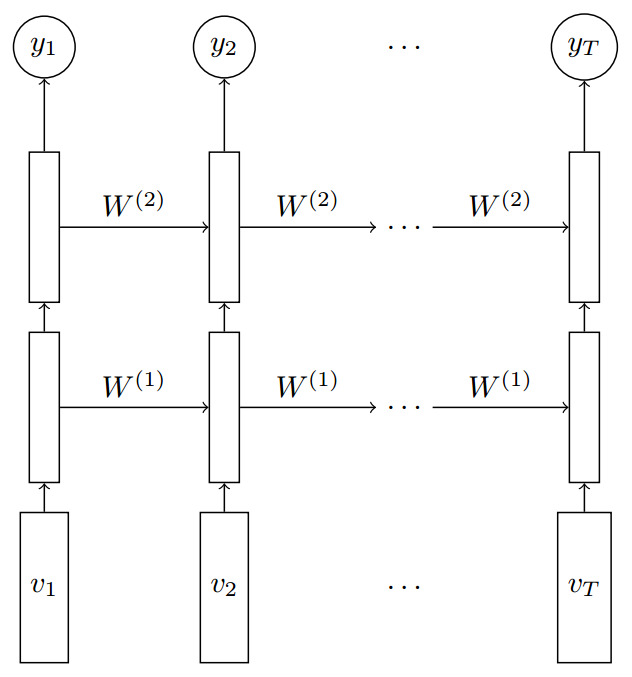
\includegraphics[width=0.7\textwidth]{img/unsupervised_learning_with_lstms_dlstm.png}
	\caption{Depiction of a \gls{dlstm} with two layers \cite{unsupervised_learning_lstms}}
	\label{fig:stateofart:unsupervised_learning_with_lstms_dlstm}
\end{figure}

For pre-training the network, the authors use a \gls{lstmsae} model. In contrast to a conventional auto encoder like described in \ref{sec:backgrund:autoencoder}, a stacked auto encoder model uses multiple encoder and decoder layers as can be seen in figure \ref{fig:stateofart:unsupervised_learning_dlstm_mts_lstmsae}. The different encoder layers are trained individually in a multi phased training procedure: Train the first auto encoder layer like a conventional \gls{lstmae} with the target being the original input data. Cut the decoder part of the first \gls{lstmae}. When training the second \gls{lstmae}, the input is encoded by both the encoder of the first and second \gls{lstmae} block and then decoded only by the decoder of the second \gls{lstmae}. The target data for training the second \gls{lstmae} is again the original input, and not the reconstructed input of the first \gls{lstmae}. The training process is depicted in figure \ref{fig:stateofart:unsupervised_learning_dlstm_mts_lstmsae}. This process is then repeated for arbitrarily many \gls{lstmae} layers. The authors tried both one and two stacked layers of \gls{lstmae}. The trained encoder blocks are then used to initialize a multi layered \gls{dlstm}.

\begin{figure}[h]
	\centering
	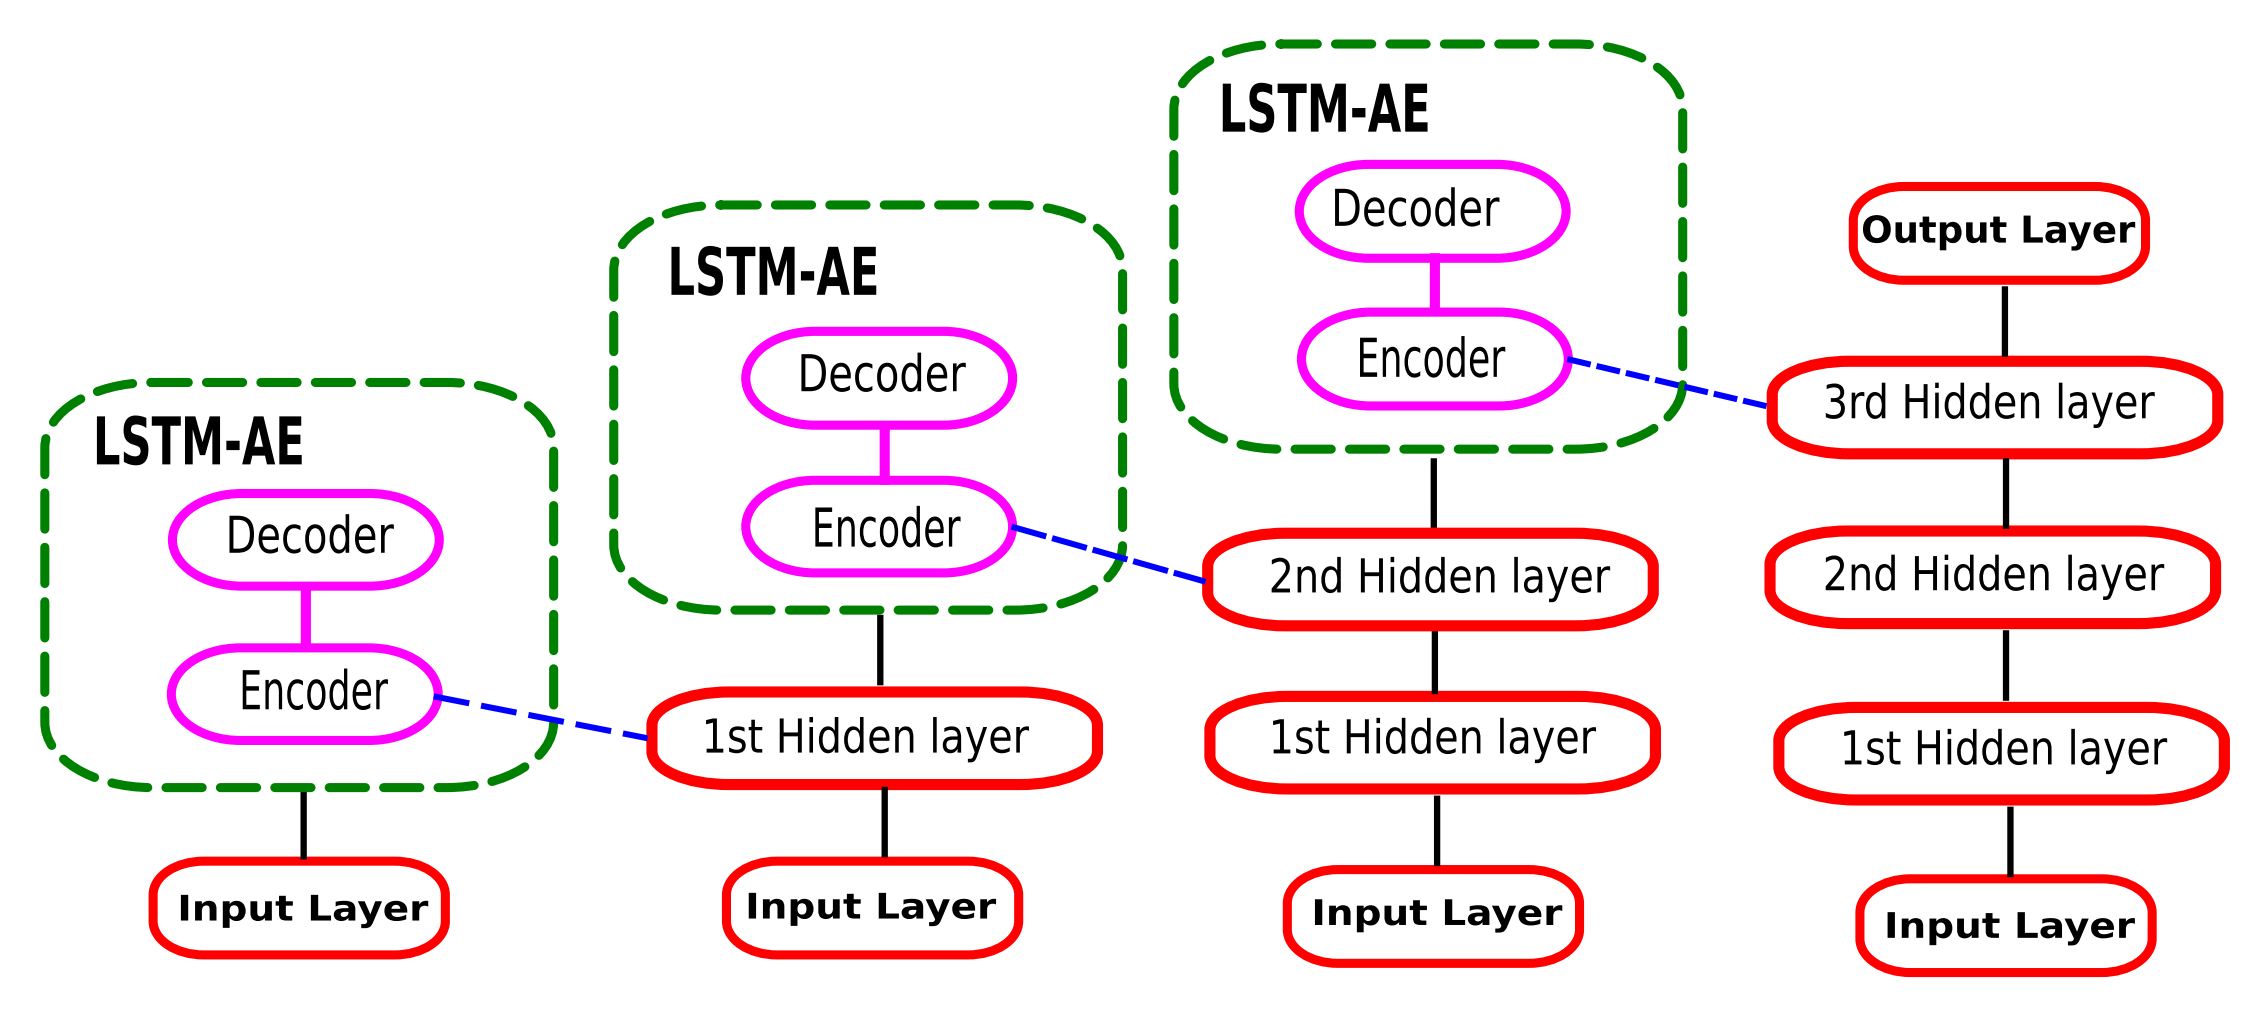
\includegraphics[width=0.9\textwidth]{img/unsupervised_learning_dlstm_mts_lstmsae.png}
	\caption{Layer-wise pre-training of \gls{lstmsae} model. \cite{unsupervised_learning_lstms_timeseries}}
	\label{fig:stateofart:unsupervised_learning_dlstm_mts_lstmsae}
\end{figure}

To complete the training phase, the parameters of the pre-trained \gls{dlstm} are then finetuned in a supervised fashion. This is done by adding an output layer which produces values of the dimension of labels of the training set used and of the variables to be predicted. In the case of the authors, the output layer was a single neuron to predict a single variable. For supervised finetuning and validation they used two datasets:

\begin{enumerate}
	\item \textit{The capital bike sharing dataset}
	\item \textit{The PM2.5 concentration in the air of CHINA dataset}
\end{enumerate}

For the first dataset, the model tried to predict how many bike will be rented on a particular day based on parameters like \textit{Season, Holiday, Weekday, Working day}, etc. For the second dataset, the task was to predict PM2.5 concentrations in the air for various Chinese cities based on parameters like \textit{Dew Point, Temperature, Pressure, Combined Wind Direction,} etc. \par

As metric of performance, the authors used \gls{rmse}, \gls{mae} and \gls{smape} (lower is better) which all describe the difference between predicted value and observed value. The results of evaluation with both data sets can be seen in tables \ref{table:stateofart:unsupervised_learning_lstms_timeseries_results1} and \ref{table:stateofart:unsupervised_learning_lstms_timeseries_results2}.

\begin{table}[]
	\begin{tabular}{l c c c c c c c}
		\thead{Model} & \thead{No. of \\ hidden
layer} & \thead{Dropout} & \thead{lag} & \thead{batch} & \thead{RMSE} & \thead{MAE} & \thead{SMAPE} \\ \hline
		\midrule
		DLSTM & 1 & 0.4 & 20 & 146 & 52.062 & 32.468 & 12.088 \\
		DLSTM & 2 & 0.3 & 25 & 219 & 49.811 & 31.524 & 12.183 \\
		LSTM-SAE & 1 & 0.1 & 30 & 219 & 49.389 & 32.192 & 13.878 \\
		LSTM-SAE & 2 & 0.1 & 30 & 73 & 46.927 & 30.041 & 11.646 \\
	\end{tabular}
	\caption{The results of \gls{dlstm} and \gls{lstmsae} using data set 1 \cite{unsupervised_learning_lstms_timeseries}}
	\label{table:stateofart:unsupervised_learning_lstms_timeseries_results1}
\end{table}

\begin{table}[]
	\begin{tabular}{l c c c c c c c}
		\thead{Model} & \thead{No. of \\ hidden
layer} & \thead{Dropout} & \thead{lag} & \thead{batch} & \thead{RMSE} & \thead{MAE} & \thead{SMAPE} \\ \hline
		\midrule
		DLSTM & 1 & 0.2 & 30 & 60 & 23.993 & 12.124 & 10.919 \\
		DLSTM & 2 & 0.2 & 30 & 73 & 23.750 & 12.452 & 12.181 \\
		LSTM-SAE & 1 & 0.1 & 30 & 219 & 23.907 & 12.509 & 11.052 \\
		LSTM-SAE & 2 & 0.3 & 25 & 146 & 24.041 & 12.060 & 9.864 \\
	\end{tabular}
	\caption{The results of \gls{dlstm} and \gls{lstmsae} using data set 2 \cite{unsupervised_learning_lstms_timeseries}}
	\label{table:stateofart:unsupervised_learning_lstms_timeseries_results2}
\end{table}

The results in tables \ref{table:stateofart:unsupervised_learning_lstms_timeseries_results1} and \ref{table:stateofart:unsupervised_learning_lstms_timeseries_results2} show that unsupervised pre-training improved final accuracy and led to better and faster convergence. \par

For this thesis, we used only a single \gls{lstmae} network, but with three layers of \gls{lstm} cells making it a \gls{dlstm} for both encoder and decoder.

\section{Machine Learning for Network Intrusion Detection}


Here provide an overview of the related state of art. Look for papers that are closest to the research you are doing
Suggestion: make a table with the related papers and compare them wrt to different criteria, for instance

\begin{itemize}
	\item Findings: What do they claim (main findings)
	\item Data: What data set they are using
	\item Methods: Which methods did they use?
	\item Reproducibility: Is it possible to reproduce the results? (e.g., is the data available? are all parameter settings provided? Is source code provided?)
	\item Relevance (How relevant is it for your work)
\end{itemize}


In the last paragraph explain how your work differs from the existing works.



\newpage

%\section{Content \& Terminology} \label{sec:content}

% insert info about previous publications below
\begin{Prev.Publ}
	Parts of the contents of this chapter have been published in the following papers:
	\begin{enumerate}
		\item [\lbrack P1\rbrack] \bibentry{cen-cenelec-etsi_smart_grid_coordination_group_smart_2014} %use the \cite ciations text
		\item [\lbrack P2\rbrack] \bibentry{enisa_smart_2014}
	\end{enumerate}
	
	Explanation text, on what parts were adopted from previous publications:\\
	e.g. "The statistical anomaly detection algorithm published in the above mentioned papers and described in this
	Chapter is based on the work done in [29]."	
\end{Prev.Publ}


\subsection{Vision \tiny{My Vision on things}} \label{subsec.vision}


\subsection{Terminology    \tiny{Architecture vs Topology + Malware vs Worm}  } \label{subsec.terminology}



\newpage
%\section{Model    \tiny{WHAT will I DO? + Abstraction}  } \label{sec:model}

% insert info about previous publications below
\begin{Prev.Publ}
	Parts of the contents of this chapter have been published in the following papers:
	\begin{enumerate}
		\item [\lbrack P1\rbrack] \bibentry{cen-cenelec-etsi_smart_grid_coordination_group_smart_2014} %use the \cite ciations text
		\item [\lbrack P2\rbrack] \bibentry{enisa_smart_2014}
	\end{enumerate}
	
	Explanation text, on what parts were adopted from previous publications:\\
	e.g. "The statistical anomaly detection algorithm published in the above mentioned papers and described in this
	Chapter is based on the work done in [29]."	
\end{Prev.Publ}

\subsection{Abstraction}
- What will be abstracted?\\
- Where do I compromise?\\


\subsubsection{Architecture} \label{subsec.architecture}
add abstraction of 4 architectures here!



\subsection{Scenarios} \label{subsec.scenarios}


\subsection{Metrics    \tiny{What do i measure?}  }


\subsection{Verification / Validation     \tiny{How do I do that??}  }
Verification: “Are we building the product right”?\\
Verification is a process of evaluating the intermediary work of a software development lifecycle to check if we are in the right track of creating the final product. Checks whether the product is built as per the specified requirement and design specification.\\

Validation: “Are we building the right product”?\\
Validation is the process of evaluating the final product to check whether the software meets the business needs. In simple words the test execution which we do in our day to day life are actually the validation activity which includes smoke testing, functional testing, regression testing, systems testing etc… It determines whether the software is fit for use and satisfy the need.

\newpage
\chapter{Methodology} \label{sec:methodology}

As summarized by the survey paper \cite{nid_ml_survey_2019} of Hongyu Liu and Bo Lang in section \ref{sec:stateofart:nid}, the design space for \gls{ml} based \gls{nids} is vast and can be hard to navigate at times. Hence, careful consideration of data representation, data pre-processing, \gls{ml} models, model parameters and training hyperparameters is necessary. The goal of the thesis was to examine the benefit of pre-training for already established \gls{dl} models in the context of \gls{nids}, hence we wanted to start from the most effective \gls{dl} models available. Derived from state-of-the-art research this seems to be a uni-directional multi-layer \gls{dlstm} in the context of \gls{nid}. Most of the state-of-the-art research on \gls{dl} however, and especially on self-supervised/unsupervised and transfer learning, is done in the context of \gls{nlp} \cite{bert}, \cite{elmo}, \cite{attention}, \cite{gpt3}. Network communication is similar to natural language in the sense that it follows a certain set of rules, a grammar so to say, and each token i.e a word or packet conveys some semantic meaning when in the context of a sentence or flow. Other researchers have made similar observations \cite{anomaly_detection_recurrent_neural_networks}. Based on the results achieved in \gls{nlp} with attention based models, we deemed the transformer encoder to be a potentially powerful new tool for network traffic classification. 

\section{Datasets} \label{sec:methodology:datasets}

We used the two \gls{nids} datasets \textit{UNSW-NB15} \cite{unsw_nb15} and \textit{CIC-IDS2017} \cite{cic_ids_2017}. \par

The \textbf{UNSW-NB15} dataset \cite{unsw_nb15}, created by Nour Moustafa et al. from the School of Engineering and Information Technology, University of New South Wales at the Australian Defence Force Academy, Australia, was released as an update for the formerly frequently used but deprecated \cite{unsw_nb15} KDD dataset family. It was designed to reflect most known low footprint attacks at time of publication. The records are bidrectional flows extracted from the raw traffic data and grouped by the commonly used \textit{<srcIP, dstIP, srcPort, dstPort, protocol>} tuple. Each flow is described by 47 derived or measured features e.g. total duration, bytes transmitted, the mean of the flow packet size transmitted by destination IP, \textit{etc}. After preprocessing where some incomplete records are removed, the dataset contains a total of 2.06 million records of which 1.99 million are normal transactions labeled as benign and 0.072 million attack records meaning 96.64\% of data is classified as benign and 3.36\% as attack. Attack records can be further divided into nine attack categories as listed in table \ref{table:methodology:datasets:unsw_nb15_categories}.

\begin{table}[H]
	\centering
	\begin{tabular}{cccccc}
		\thead{\textbf{\#}} & \thead{\textbf{Class}} & \thead{\textbf{\textbf{No. Records}}} & \thead{\textbf{\% w.r.t.} \\ \textbf{benign class}} & \% \thead{\textbf{\% w.r.t.} \\ \textbf{majority atk. class}} & \thead{\textbf{\% w.r.t.} \\ \textbf{total instances}} \\ \hline \midrule
		0  & Analysis       & 534         & 0.03\%                 & 1.82\%                        & 0.03\%                    \\ \midrule
		1  & Backdoors      & 397         & 0.02\%                 & 1.36\%                        & 0.02\%                    \\ \midrule
		2  & DoS            & 3972        & 0.20\%                 & 13.57\%                       & 0.19\%                    \\ \midrule
		3  & Exploits       & 29281       & 1.47\%                 & 100.00\%                      & 1.42\%                    \\ \midrule
		4  & Fuzzers        & 20848       & 1.05\%                 & 71.20\%                       & 1.01\%                    \\ \midrule
		5  & Generic        & 4301        & 0.22\%                 & 14.69\%                       & 0.21\%                    \\ \midrule
		6  & Benign         & 1991349     & 100.00\%               & 6800.82\%                     & 96.46\%                   \\ \midrule
		7  & Reconnaissance & 11971       & 0.60\%                 & 40.88\%                       & 0.58\%                    \\ \midrule
		8  & Shellcode      & 1546        & 0.08\%                 & 5.28\%                        & 0.07\%                    \\ \midrule
		9  & Worms          & 185         & 0.01\%                 & 0.63\%                        & 0.01\%                   
	\end{tabular}
 	\caption{UNSW-NB15 dataset record distribution \cite{unsw_nb15}.}
 	\label{table:methodology:datasets:unsw_nb15_categories}
\end{table}

The dataset was generated from a synthetic environment comprised of 3 networks and 45 distinct IP addresses using the IXIA PerfectStorm (now keysight PerfectStorm) tool.

The \textbf{CIC-IDS2017} dataset \cite{cic_ids_2017}, created by Iman Sharafaldin et. al from Canadian Institute for Cybersecurity (CIC), University of New Brunswick (UNB), Canada constitutes another updated representation of known attack types at the time of publication. Compared to the UNSW-NB15 dataset it contains records of more modern cyber attacks like Heartbleed, HULK DoS but leaves out e.g. worm attacks. It contains a total of 2.31 million records of which 1.73 million are labeled as benign and 0.58 million are attack records. In other words, 74.72\% of the dataset are benign records and 25.28\% attack records. Attack records are further classified as shown in table \ref{table:methodology:datasets:cic_ids_2017_categories}.

\begin{table}[H]
	\centering
	\begin{tabular}{cccccc}
		\thead{\textbf{\#}} & \thead{\textbf{Class}} & \thead{\textbf{No. Records}} & \thead{\textbf{\% w.r.t.} \\ \textbf{benign class}}s & \thead{\textbf{\% w.r.t.} \\ \textbf{majority atk. class}} & \thead{\textbf{\% w.r.t.} \\ \textbf{total instances}} \\ \hline \midrule
		0  & Botnet ARES             & 755         & 0.04\%                 & 0.32\%                          & 0.03\%                    \\ \midrule
		1  & FTP-Patator             & 254         & 0.01\%                 & 0.11\%                          & 0.01\%                    \\ \midrule
		2  & SSH-Patator             & 2,556        & 0.15\%                 & 1.09\%                          & 0.11\%                    \\ \midrule
		3  & DDoS LOIT               & 94,327       & 5.46\%                 & 40.39\%                         & 4.08\%                    \\ \midrule
		4  & DoS GoldenEye           & 7,451        & 0.43\%                 & 3.19\%                          & 0.32\%                    \\ \midrule
		5  & DoS Hulk                & 233,521      & 13.53\%                & 100.00\%                        & 10.11\%                   \\ \midrule
		6  & DoS Slowhttptest        & 4,209        & 0.24\%                 & 1.80\%                          & 0.18\%                    \\ \midrule
		7  & DoS slowloris           & 3,886        & 0.23\%                 & 1.66\%                          & 0.17\%                    \\ \midrule
		8  & Heartbleed              & 2           & 0.00\%                 & 0.00\%                          & 0.00\%                    \\ \midrule
		9  & Infiltration            & 76,237       & 4.42\%                 & 32.65\%                         & 3.30\%                    \\ \midrule
		10 & Benign                  & 1,726,226     & 100.00\%               & 739.22\%                        & 74.72\%                   \\ \midrule
		11 & PortScan - Firewall off & 159,648      & 9.25\%                 & 68.37\%                         & 6.91\%                    \\ \midrule
		12 & PortScan - Firewall on  & 381         & 0.02\%                 & 0.16\%                          & 0.02\%                    \\ \midrule
		13 & SQL Injection           & 13          & 0.00\%                 & 0.01\%                          & 0.00\%                    \\ \midrule
		14 & XSS WebAttack           & 678         & 0.04\%                 & 0.29\%                          & 0.03\%                   
	\end{tabular}
	\caption{CIC-IDS2017 dataset record distribution \cite{cic_ids_2017_analysis}.}
	\label{table:methodology:datasets:cic_ids_2017_categories}
\end{table}

In contrast to the UNSW-NB15 network simulation environment, the network topology consists of two networks: A highly secured victim network with firewall, router, switches and most common operating systems and a separated attack network containing a set of PCs with public IPs and running Windows 8.1 and Kali Linux.

To reduce variance in results and to keep comparability high we use the same random seed for all experiments and use stratified sampling when we divide the data sets into smaller chunks for pre-training, training and validation to assure the each attack category is represented in the subset proportionally to the whole dataset. This is especially important if we use very small subsets (10 flows per attack category) for fine-tuning as described in section \ref{sec:experiments}. 

\subsection{Subsets} \label{sec:methodology:subsets}

Pre-training and training in our experiments is conducted on subsets of the original dataset i.e. 80\% for pre-training, 10\%, 1\% and even smaller splits for fine-tuning. The split of the datasets is performed by stratified sampling so the ratio of each attack class stays roughly the same in the different splits as in the original dataset. \par

In hope of making any possible positive results more salient, we devised an extreme scenario where we limit the labeled date available for fine-tuning to a bare minimum of 10 records at most (for some categories, the dataset contains less than 10 samples) per attack category present in the original dataset. We then include an amount of benign records to keep the ratio of attack/benign flows of the original dataset. This results in the two subsets elaborated in tables \ref{table:methodology:datasets:cic17_subset} and \ref{table:methodology:datasets:unsw15_subset} labeled \textbf{CIC17\_10} and \textbf{UNSW15\_10} for the corresponding datasets.

\begin{table}[H]
	\centering
	\begin{tabular}{ccc}
		\thead{\textbf{\#}} & \thead{\textbf{Class}} & \thead{\textbf{No. Records}} \\ \hline \midrule
		0  & Botnet ARES             & 10  \\
		1  & FTP-Patator             & 10  \\
		2  & SSH-Patator             & 10  \\
		3  & DDoS LOIT               & 10  \\
		4  & DoS GoldenEye           & 10  \\
		5  & DoS Hulk                & 10  \\
		6  & DoS Slowhttptest        & 10  \\
		7  & DoS slowloris           & 10  \\
		8  & Heartbleed              & 10  \\
		9  & Infiltration            & 10  \\
		10 & Benign                  & 391 \\
		11 & PortScan - Firewall off & 10  \\
		12 & PortScan - Firewall on  & 10  \\
		13 & SQL Injection           & 1   \\
		14 & XSS WebAttack           & 10                    
	\end{tabular}
	\caption{Subset \textbf{CIC17\_10} devised for CIC-IDS2017 to include a minimal amount of records amounting to approximately 0.023\% of the total dataset.}
	\label{table:methodology:datasets:cic17_subset}
\end{table}

\begin{table}[H]
	\centering
	\begin{tabular}{ccc}
		\thead{\textbf{\#}} & \thead{\textbf{Class}} & \thead{\textbf{\textbf{No. Records}}} \\ \hline \midrule
		0 & Analysis       & 10     \\
		1 & Backdoors      & 10     \\
		2 & DoS            & 10    \\
		3 & Exploits       & 10   \\
		4 & Fuzzers        & 10   \\
		5 & Generic        & 10    \\
		6 & Benign         & 2543 \\
		7 & Reconnaissance & 10   \\
		8 & Shellcode      & 10    \\
		9 & Worms          & 10                     
	\end{tabular}
	\caption{Subset \textbf{UNSW15\_10} devised for UNSW-NB15 to include a minimal amount of records amounting to approximately 0.11\% of the total dataset.}
	\label{table:methodology:datasets:unsw15_subset}
\end{table}

\section{Data Representation}

Network traffic data can be viewed from a multitude of perspectives ranging from aggregate statistical data over different time-frames \cite{kitsune} to looking at feature representations of single packets. These can be viewed in the context of \textit{flows}.
Flows are loosely defined as sequences of packets that share a certain property \cite{adversarial_recurrent_ids}. In our case we define flows as sequences of packets that share source and destination IP address, source and destination port, and the network protocol used. This creates the quintuple \textit{<srcIP, dstIP, srcPort, dstPort, protocol>} as the key over which individual packets are aggregated to flows, which is a very common approach \cite{caia_vector}, \cite{unsw_nb15}, \cite{feature_vectors}. We chose a flow representation since this approach has shown good results frequently, is easy to obtain, requires no domain knowledge and is feasible for encrypted traffic \cite{feature_vectors}. We decided not to include any packet payload features except the packet length in bytes, as in a real world scenario most of the traffic would be encrypted anyway. This leads to poor classification performance for \gls{u2r} and \gls{r2l} \cite{nsl_kdd} like SQL injection, XSS and other payload based attacks which is also shown by our results as can be seen in section \ref{sec:results}. Commonly, flows are represented as a single feature vector in the dataset, containing aggregated statistical data of the completed flow like e.g. the mean of the flow packet size transmitted by the source IP, source to destination packet count or bits per second or total duration of the transmission. However, we use a packet sequence representation instead of an aggregate flow tensor due to its similarity with natural language as mentioned before, which enables us to apply state-of-the-art methods and sequence2sequence models from \gls{dl} based \gls{nlp}. 

%The downside of this is that flows can be processed only once they are completed \cite{adversarial_recurrent_ids}. In a real world scenario, this approach has major downsides since the \gls{ids} can only inspect communications in retrospect and never in real time, since its not feasible to recalculate all features in the flow vector after . This was one of the reasons we decided to represent our flows as a sequence of packets instead of a single aggregated feature vector. Each packet is represented by the 15 features in table \ref{table:methodology:data_representation:features}.

\begin{table}[h]
	\centering
	\begin{tabular}{c c c c l}
		\thead{\textbf{\#}} & \thead{\textbf{Name}} & \thead{\textbf{Type}} & \thead{\textbf{Constant} \\ \textbf{over flow}} & \thead{\textbf{Description}} \\ \hline \midrule
		0 & srcPort & Int & yes & Source port number \\ \midrule
		1 & dstPort & Int & yes & Destination port number \\ \midrule
		2 & protocol & Int & yes & IP protocol identifier \\ \midrule
		3 & pktLength & Int & no & Packet length in bytes \\ \midrule
		4 & pktIat & Int & no & \gls{iat} \\ \midrule
		5 & pktDirection & Bool & no & Sending direction of the packet \\ \midrule
		6 & synFlag & Bool & no & TCP SYN Flag \\ \midrule
		7 & finFlag & Bool & no & TCP FIN Flag \\ \midrule
		8 & rstPort & Bool & no & TCP RST Flag \\ \midrule
		9 & pshFlag & Bool & no & TCP PSH Flag \\ \midrule
		10 & ackFlag & Bool & no & TCP ACK Flag \\ \midrule
		11 & urgFlag & Bool & no & TCP URG Flag \\ \midrule
		12 & eceFlag & Bool & no & TCP ECE Flag \\ \midrule
		13 & cwrFlag & Bool & no & TCP CWR Flag \\ \midrule
		14 & nsFlag & Bool & no & TCP NS Flag \\ \midrule
	\end{tabular}
	\caption{Packet features \cite{cic_ids_2017_analysis}.}
	\label{table:methodology:data_representation:features}
\end{table}

The sending direction \textit{pktDirection} of the packet is a binary feature where $0$ is the direction of the first packet in the flow and $1$ is the complementary direction. \par

We used the data pre-processing from the paper \cite{adversarial_recurrent_ids} by Tanja Zseby et al. as it fit the requirements for our experiments and was easily modifiable. Starting from captured network traffic in the form of PCAP files, we used the tool go-flows \cite{go_flows} to extract the specified features and used the same python script as was used for the experiments in the paper \cite{adversarial_recurrent_ids} to assign labels to the extracted flows. \par

To keep gradient paths shorter and to improve training stability, packet sequences are truncated to be at most 100 packets long. As last step of pre-processing features are min-max normalized to be within a range of $[-1,1]$ to make gradient descent converge quicker. \par

\begin{figure}[h]
	\centering
	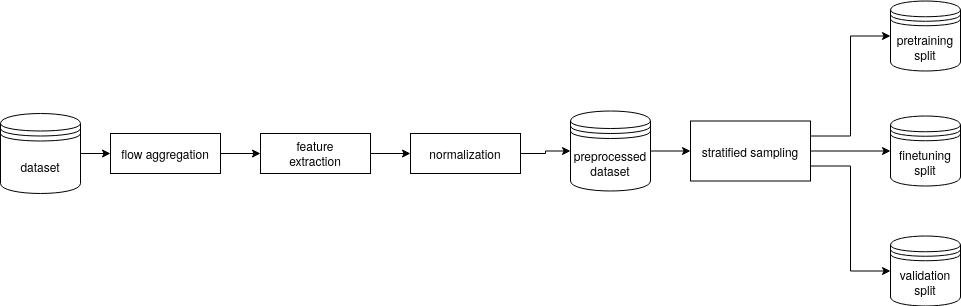
\includegraphics[width=0.95\linewidth]{graphics/img/dataset_preprocessing.png}
	\caption{All steps performed in dataset preprocessing to yield pre-training, training and validation splits.}
	\label{fig:dataset_preprocessing}
\end{figure}

\section{Machine Learning Models}

To inspect the potential benefits of self-supervised pre-training for \gls{ml}-based intrusion detection we chose to take a look at \gls{lstm} and networks as they are suited to process sequences of variable length and have shown promising results in the past in the domains of \gls{ids} and/or \gls{nlp} \cite{bert}, \cite{attention_model_ids}. Both types of networks are generally susceptible to improvements through self-supervised pre-training as prior research has shown \cite{bert} \cite{unsupervised_learning_lstms} \cite{unsupervised_learning_lstms_timeseries}. Whether pre-training improves performance in the context of \gls{nids} remains to be shown and is subject of this thesis.

For our \textbf{\gls{lstm} network} we chose a three layer \gls{dlstm} with a \textit{hidden size} of 512. While a larger network might be slightly more effective, this configuration proved to be swiftly trainable while also producing results close to those achieved by other researchers using \gls{lstm} models applied to the same datasets \cite{fog_based_detection_survey_2020}. A depiction of the data flow and layers of a three layered \gls{lstm} can be seen in figure \ref{fig:stateofart:unsupervised_learning_with_lstms_dlstm}. \par

Since our main focus is on comparisons between different training methods applied to the same model, it is not necessary to achieve optimal results as this would unnecessarily increase the training time needed until the model converges. For training the \gls{lstm} model, each flow is considered one sample and each packet is one token. The tokens are processed by the model in chronological order, meaning packets with an earlier timestamp will be processed first. The timestamp however is not part of the feature representation but is considered for data pre-processing to order packets within flows. \par
Independent of the context, \gls{lstm} models have shown to be sensible to initialization of their weights and hidden state. This can be seen as a drawback but also as an opportunity to increase performance or decrease learning time. While there are many ways to initialize the weights of an \gls{lstm} network, the most common ones are random initialization, orthogonal initialization or some form of transfer learning which in our case is self-supervised pre-training. \par
For pre-training, the output layer is a linear layer with 15 nodes, equal to the number of features, and no activation function. This is necessary as for pre-training the output of the model is a sequence of feature vectors representing network packets e.g. when calculating the identity function the model is tasked with producing the input packet sequence as the model output. For binary classification the output layer is replaced with a linear layer with a single node because only one bit of information is needed to distinguish between \textit{attack} and \textit{no-attack}. The node has no activation function on its own because we use the PyTorch implementation \textit{torch.nn.BCEWithLogitsLoss} of \gls{bce} which applies a sigmoid activation function as first step of the calculation. This results in a sequence2sequence model which generates output sequences equal to the length of the input sequence. For supervised fine-tuning the target sequence is one of length $n$ equal to the input sequence length where every element is the target label of the binary classification e.g. if the sequence is classified as an attack the target label would be $1$ and the target sequence for supervised training would be $y^{(t)} = (1,...,1)$ of length $n$. For validation however it would only require a sequence2scalar model so only the output of the last stage is looked at because at that point, the whole input sequence was processed by the model and information in a (uni-directional) \gls{lstm} only flows in one direction. The output of this stage should therefore be most accurate.

\begin{figure}[h]
	\centering
	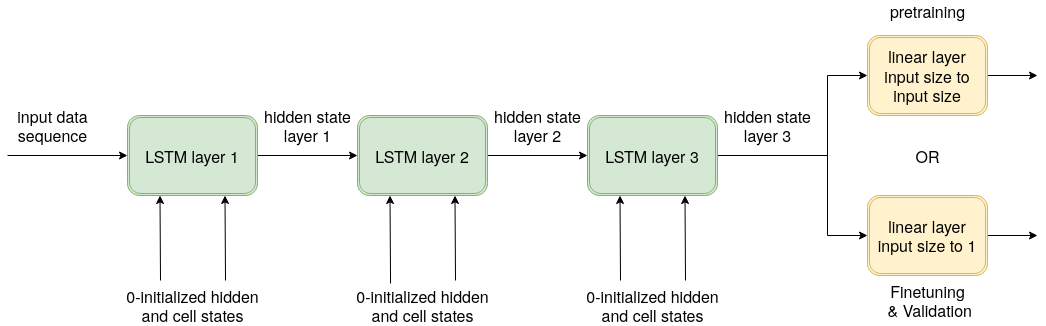
\includegraphics[width=0.95\linewidth]{graphics/img/lstm_model.png}
	\caption{Depiction of the \gls{lstm} model.}
	\label{fig:lstm_model}
\end{figure}

The  model as proposed by Vaswani et. al \cite{attention} and its derivative score high on the leader boards of \gls{nlp} benchmarks like GLUE \cite{glue} or SQuAD \cite{bibid} and are still considered state-of-the-art in many regards. Following the example of \gls{bert} we only used the encoder part of the \textit{ network} since the decoder does not provide any benefits for classification problems. We tuned the model parameters to be 10  layers, each layer consisting of a 3-headed Multi-Head Attention block and a feed-forward network with a forward expansion of 2, meaning an internal representation size double to the number of features per packet. For pre-training, the output layer is a linear layer with 15 nodes, equal to the number of features, and no activation function. For binary classification the output layer is replaced with a linear layer with a single node and no activation function because the objective function for binary classification \gls{bce} loss operates on logits. This again results in a sequence2sequence model which produces output sequences of length equal to the input sequence. For binary classification, we only need a single value, but the  Encoder model produces a sequence of values. In contrast to the \gls{lstm} model, information in the  does not aggregate at a specific stage and therefore we can't identify an output token which has more information or is more likely to be accurate than others. Google solved this problem for \gls{bert} by prepending a classification token to every input sequence and the model learns to aggregate information regarding classification at the corresponding output token. We tried this approach with no success, perhaps due to insufficient training. We opted for an average pooling layer over all output tokens to get from a sequence of variable length to a single value and this approach also works as can be seen later in the results section \ref{sec:results:transformer}.

\todo{insert image of transformer model} 

\section{Framework and Training} \label{sec:methodology:freamework_and_training}

To conduct our experiments we used PyTorch \cite{pytorch} to implement and train our proposed models. To save labor and to keep results comparable we used the standard implementations \textit{torch.nn.LSTM} and \textit{torch.nn.Encoder}. Training is conducted by a standard training loop going through forward and back propagation, calculating losses and updating weights for each batch. Noteworthy is the use of gradient clipping to a maximum of 1 and the use of a learning rate scheduler which decreases the learning rate by a factor of 0.1 if mean batch loss is plateauing during training. As optimization criterion for pre-training we use L1 loss, i.e. \gls{mae} (\textit{nn.L1Loss}). For supervised training we use \gls{bce} loss with mean reduction on logits directly (\textit{nn.BCEWithLogitsLoss}).
For updating weights we use the \textit{Adam} optimizer \cite{adam} which is an extension to the commonly used \gls{sgd} method. Similar to \textit{AdaGrad} \cite{optimizer_comparison} and \textit{RMSProp} \cite{optimizer_comparison} it maintains separate learning rates for each individual weight instead of using the same learning rate for every weight like in classic \gls{sgd}. Compared to other optimizers \textit{Adam} was shown to be more effective in improving training efficiency \cite{adam} and is appropriate for noisy or sparse gradients which can occur when working with \glspl{rnn} in general.
We developed and implemented a framework in Python to automate the experiments, generate statistics, plots and metrics. \par
The models were trained on two NVidia GeForce RTX 2070 Super GPUs with a combined performance of 19.4 Teraflops per second for 32bit float (FP32) values. For some instances, i.e. for pre-training with the proxy tasks MASK on the transformer model and for pre-training with the proxy task IDENTITY and PREDICT we use 16bit float (FP16) values during training together with the \textit{torch.cuda.amp.GradScaler}. This significantly decreases training time and GPU load but introduced numerical instability in some cases and for most cases we went back to training with FP32 values. Training was performed with a batch size of 128 for the \gls{lstm} model and 1024 for the Encoder model. Further increasing batch size did not improve final accuracy nor did it decrease the time in which training converges. \par

\section{Metrics and Validation}

All tables, graphs and plots are automatically generated by a results script which trains the models with parameters set in a configuration file and generates the necessary data for all subsequent analysis methods i.e. performance metrics, per attack class statistics, \gls{pdp}, neuron activation plots and \gls{dtc}. It subsequently generates latex tables and graphical elements which are included in this thesis. During supervised training the model is validated every 6, 2 and 1 epoch(s) for trainings with a total of 600, 200 and 100 training epochs respectively. The metrics described in section \ref{sec:background:metrics} are generated and stored for every validated epoch. The results in the following sections and all plots are generated with the model from the epoch with the highest recorded accuracy score. Hence, the tables in the results chapter \ref{sec:results} also include the number of the training epoch after which the numbers where generated and the training time needed on the setup described in the previous section \ref{sec:methodology:freamework_and_training} to reach that epoch.
\newpage
\chapter{Experiments}\label{sec:experiments}

To inspect the potential benefits of self-supervised pre-training for \gls{ml}-based intrusion detection we chose to take a look at \gls{lstm} and the Transformer networks as they are suited to process data of variable length and have shown promising results in the past \todo{give examples}. Network traffic data can be looked at from a multitude of perspectives ranging from aggregate statistical data over different time-frames \cite{kitsune} to looking at a feature representation of single packets which can be looked at in the context of \textit{flows}. Flows are loosely defined as sequences of packets that share a certain property \cite{adversarial_recurrent_ids}. In our case we define flows as packets that share source and destination IP address, source and destination port, and the network protocol used. This creates the quintuple \textit{<srcIP, dstIP, srcPort, dstPort, protocol>} as the key over which individual packets are aggregated to flows. We used the data pre-processing from \cite{adversarial_recurrent_ids} as it fit the requirements for our experiments and was easily modifiable. The underlying data from which flow data is extracted are the \textit{CIC-IDS-2017} \cite{cic_ids_2017} and \textit{UNSW-NB15} \cite{unsw_nb15} \gls{nids} datasets. After the data pre-processing from \cite{adversarial_recurrent_ids} each packet is represented by source port, destination port, packet length, \gls{iat}, packet direction and all TCP flags (SYN, FIN, RST, PSH, ACK, URG, ECE, CWR, NS) resulting in 15 input features to be used in training the \glspl{nn}. \par

The task of the \glspl{nn} is to classify each flow into either \textit{benign} or \textit{attack} which results into a binary classification problem. Ordinary network traffic that should be ignored by the \gls{ids} is labeled as \textit{benign} and flows that constitute or are part of a cyber-attack are labeled as \textit{attack}. As there are only two possible labels, \gls{bce} can be used as loss function to determine the distance between the predicted label by the \glspl{nn} and the actual label \todo{give more detailed explaination of BCE Loss}. For updating weights we use the \textit{Adam} optimizer \cite{adam} which is an extension to the commonly used \gls{sgd} method. Similar to \textit{AdaGrad} \cite{optimizer_comparison} and \textit{RMSProp} \cite{optimizer_comparison} it maintains separate learning rates for each individual weight instead of using the same learning rate for every weight like in classic \gls{sgd}. Compared to other optimizers \textit{Adam} was shown to be more effective in improving training efficiency \cite{adam} and is appropriate for noisy or sparse gradients which can occur when working with \glspl{rnn} in general.

As a premise for our research we trained the \gls{lstm} and the Transformer network in a solely supervised fashion to get a baseline the pre-training results can be compared to. Supervised training was performed for 10 epochs each for 90\%, 5\% and 1\% of available data and a constant 10\% of data for validation which has not been used for training. We specifically wanted to know how the networks would perform in a scenario where very little labeled training data was available as this would best describe a scenario where large amounts of unlabeled data are available for self-supervised pre-training and only a small amount of labeled data for fine tuning. To pre-train a \gls{nn} the network is given a task that is not necessarily connected to the final purpose of the network, often referred to as a \textit{proxy task}. By solving the proxy task the network attempts to find structure in the data and should learn to form a more abstract representation of the data within its latent space. E.g. with \gls{bert} pre-training is performed by masking a certain percentage of the input and having the \gls{nn} predict the missing words and additionally letting the network guess whether one sentences precedes another in a text. We defined our own proxy tasks for pre-training the networks as described in the following sections.


\section{Self-supervised Pre-training for Long Short-Term Memory Networks} \label{sec:experiments_lstm}

For our \gls{lstm} network we chose a three layer \gls{lstm} with a \textit{hidden size} and \textit{cell size} of 512. While a larger network might be more effective, this configuration proved to be swiftly trainable while also producing results close to the optimum \todo{provide numbers}. Since we are only interested in comparisons between different training methods applied to the same model, it is not necessary to increase model size to achieve optimal results as this would unnecessarily increase the training time needed until the model converges. For training the \gls{lstm} model, each flow is considered one sample and each packet is one token. The tokens are processed by the model in chronological order, meaning packets with an earlier timestamp will be processed first. The timestamp however is not part of the feature representation but is considered for data pre-processing to order the packets within the flow. For pre-training the \gls{lstm} we devised three different proxy tasks for the model to solve in a self-supervised fashion: Predicting the next packet in the flow, predicting masked features where the same feature is masked in every packet of the sample and predicting randomly masked packets. The \gls{mae} is used to determine the error between prediction and target data. Translating to PyTorch this means we used \textit{L1Loss} with \textit{mean} reduction as the loss function for pre-training. We tuned the hyper-parameters of training for both supervised and self-supervised training to an initial \textit{learning rate} of $10^{-3}$ and a \textit{batch size} of 128. Over the training process, the learning rate will be adjusted by Adam so the model is robust to changes on the initial learning rate. 

\subsection{Predict Packet} \label{sec:experiments_lstm_predict_packet}

For this proxy task, the model has to predict the next packet in the flow. We started by predicting only the last packet in each flow but then moved to predicting all packets in a flow except the first. This means having a \textit{sequence-to-sequence} model where the inputs are all tokens in one flow except the last, because it has no successor. The target data are all tokens in the same flow except the first, because it has no predecessor. This results in two comparable tensors of equal length $n-1$ where $n$ is the original sequence length of the flow. This way, a lot more information is conveyed to the network when compared to only predicting the last packet in a flow. At first glance, this looks similar to Auto-Encoding. The key difference is however, that the token which is to be predicted is not yet available as an input token to the model, meaning it has to derive the features by other means than conveying the requested input token to the output. The loss is calculated as the \gls{mae} (\textit{L1Loss} with \textit{mean} reduction) between the predicted logits and the target data sequences.

\subsection{Mask Features} \label{sec:experiments_lstm_mask_feature}

For this pre-training task, the model is to predict masked features of some packets in the sequence. We have tried multiple masking values but -1 produces the best results out of the values we tried \todo{give a comparison of values}. This proxy task in particular can be parameterized in different ways. E.g. the number of features and which features to mask, if always the same features are masked or if the selection is random for each packet or for each flow, if every packet in the sequence has some masked features or if there is only a chance that a packet is selected for masking. Those are only some examples of how this task can be set up in different ways. To be completely exhaustive was not possible, so we compiled a selection of some of the variations as an overview of the parameter space. For pre-training the model the masked data is provided as input sequence and the unmasked data is the target. The loss is calculated as the \gls{mae} (\textit{L1Loss} with \textit{mean} reduction) between the predicted logits and the target data sequences. \todo{enumerate all parameter combinations}

\subsection{Mask Packets} \label{sec:experiments_lstm_mask_packet}

Similar to the pre-training in \gls{bert}, all features of random packets in the sequence are masked with a value of -1 and the model is to predict the masked tokens. Again, \gls{mae} is used as the loss function. Unlike to \gls{bert}, we don't only look at the masked tokens when calculating the loss but compare every feature of every packet, also the non-masked ones, which adds an auto-encoding property to the pre-training. We found this to have more beneficial effect on the results than only looking at the masked packets. The most important parameter here is the ratio of how many packets per sequence are to be masked compared to its sequence length. To work with an absolute number of masked packets is not feasible as sequence length varies from 1 to a set max sequence length which in our case was 100. If an absolute number was used to determine how many packets should be masked some sequences would be completely masked out which would not be beneficial for training.

\section{Self-supervised Pre-training for Transformer Networks} \label{sec:experiments_transformer}

Following the example of \gls{bert} we only used the encoder part of the transformer since the decoder does not provide any benefit for classification problems. We tuned the model parameters to be 10 Transformer layers, each layer consisting of a 3-headed Multi-Head Attention block and a feed-forward network with a forward expansion of 20 times the input size, i.e. the number of features per packet. Since we did not observe any over-fitting during training, we set the drop-out rate to zero (except for training with the Auto-Encoder \ref{sec:experiments_transformer_autoencoder}). 
Like with the \gls{lstm} we devised a series of proxy tasks for pre-training the model in self-supervised fashion. Since the information flow is different in Transformers than it is in \glspl{lstm}, the pre-training task \textit{Predict Packets} \ref{sec:experiments_lstm} we used for the \gls{lstm} is no longer feasible. While the \gls{lstm} at each stage has only access to all the tokens it processed up to this point, the Transformer has access to all input tokens at each stage of the execution which is one of the benefits of self-attention \cite{attention}. Contrary to our expectations, supervised training on the Transformer takes longer than on the \gls{lstm} to achieve the observed optimal accuracy of 99,65\%. In other words, when training the \gls{lstm} and the Transformer network for the same amount of time, the \gls{lstm} produces better results. In the following sections we describe the pre-training methods we used for to pre-train the Transformer network.

\subsection{Mask Features} \label{sec:experiments_transformer_mask_features}

Analogous to the \textit{Mask Features} proxy task for the \gls{lstm}, we used the same method for pre-training the Transformer.

\subsection{Autoencoder} \label{sec:experiments_transformer_autoencoder}

Autoencoder are an established concept when it comes to self-supervised learning \todo{give some examples}. With this method input and target data are the same and the network is tasked with reconstructing the input data at the output. To prevent the network from simply "transporting" the input tokens through the network without having to learn anything, a form of regularization is introduced to force the network into learning an abstract representation of the data \cite{autoencoders}. 
In our case, we used the dropout rate to introduce artificial noise into the input data.

\subsection{Mask Packet}

For this proxy task, random packets in the flow are masked with a value of -1 and the model is to predict only the masked packets. Since a packet in a flow can be seen as a word in a sentence, and the feature representation of a packet is similar to an embedded word vector, this pre-training method is analogous to the method to pre-train the \gls{bert} model. 

\newpage

\chapter{Results} \label{sec:results}

In this chapter, we present the results from experiments proposed in the previous chapter. Like with the experiments section, we will be looking at the results from \gls{lstm} and the transformer model independently. An in-depth look into the datasets and the workings of the differently trained models based on \gls{pd} plots, neuron data plots and the outputs of a fitted \gls{dtc} follow in the section \ref{sec:results:explainability}.

\section{Long Short-Term Memory Model} \label{sec:results:lstm}

As a baseline, we look at results where the model has been trained in a purely supervised fashion with different amounts of data of the two datasets. The results are comparable to previous experiments with deep neural networks on these datasets \cite{fog_based_detection_survey_2020} and even slightly better in some instances. Looking at tables \ref{table:results:lstm:stats_flows_supervised}, \ref{table:results:lstm:stats_flows15_supervised} we can already see that very little supervised data is needed to achieve fairly high accuracy. For the \gls{lstm} model, going from 90\% of training data (exp. 1.1.1 and 1.2.1) to 10\% (exp. 2.1.1 and 2.4.1) only amounts to an absolute drop of 0.164\% and 0.276\% accuracy for CIC-IDS2017 and UNSW-NB15 datasets respectively. Most astounding are also the results when dropping from millions of records when training with 90\% of the datasets to just the specialized subsets containing a couple of hundred entries in total and only 10 records of each attack class. Withholding most of labeled data in the datasets, this constraint only amounts to an absolute accuracy decrease of 4.114\% and 1.176\% for datasets CIC-IDS2017 and UNSW-NB15 respectively.
While this is fairly pleasant in general, it means that results will be harder to improve as any benefit pre-training provides might be overshadowed by the effectiveness of supervised training, even with very little data. \par

\input{results/results/rn500/lstm/tables/flows_supervised/stats_comparison_ALL}

\input{results/results/rn500/lstm/tables/flows_supervised/class_comparison_ALL}

Next, we will be looking at results for pre-training with the different proxy tasks and different amounts of data used for supervised finetuning. Tables \ref{table:results:lstm:stats_flows_10}, \ref{table:results:lstm:stats_flows_1} and \ref{table:results:lstm:stats_flows_subset} show results for experiments 2.1.1 - 2.1.6, 2.2.1 - 2.2.6 and 2.3.1 - 2.3.6 on dataset CIC-IDS2017 conducted with 10\%, 1\% and only a very small fraction of data as defined in subset CIC17\_10. Looking at the performance metrics, we can see that there is some variance in the resulting data. The NumPy and PyTorch random seeds are the same for all experiments which means that pre-training, supervised finetuning and validation have been conducted with the exact same subsets of the original dataset which means that differences in results can only come from pre-training with different proxy tasks. This establishes the fact that pre-training in general, and also different methods of pre-training have an effect on final performance. Starting with table \ref{table:results:lstm:stats_flows_10}, we can see that pre-training with some proxy tasks improves performance while others have almost no effect or even a negative effect. \par

\input{results/results/rn500/lstm/tables/flows15_supervised/stats_comparison_ALL}

\input{results/results/rn500/lstm/tables/flows15_supervised/class_comparison_ALL}

For accuracy, the highest positive delta 0.101\% in experiments 2.1.1-6 in table \ref{table:results:lstm:stats_flows_10} can be observed for pre-training with the COMPOSITE proxy task \ref{sec:experiments:lstm:composite} closely followed by pre-training with the ID proxy task \ref{sec:experiments:lstm:identity} with a delta of 0.095\%. The highest negative delta in accuracy, -0.010\%, can be observed for the OBSCURE feature proxy task \ref{sec:experiments:lstm:obscure}. It should be noted, that for detection rate, the highest delta is 0.343\% also occurring after COMPOSITE pre-training. This shows that the improvement in accuracy stems from improved attack detection capability achieved through pre-training. \par

\input{results/results/rn500/lstm/tables/flows_10/stats_comparison_ALL}

\input{results/results/rn500/lstm/tables/flows_10/class_comparison_ALL}

Looking at table \ref{table:results:lstm:stats_flows_1} we can inspect for which attack categories improvement is most salient. When comparing training with supervised methods only in experiment 2.1.1 with the on the COMPOSITE proxy task pre-trained model in experiment 2.1.6 we can see major improvements for detection of FTP-Patator brute force attacks. Accuracy jumped from 72\% for supervised only training to 92.308\% for the COMPOSITE trained model and even 96.154\% for the PREDICT proxy task, constituting a positive delta of 24.154\%. For experiment 2.1.4, pre-training with the auto encoder task, the accuracy for detection of the FTP-Patator attack category dropped to 3.846\%. Such high variance in results shows again that the \gls{lstm} model is susceptible to different pre-training strategies. Other attack classes which have seen improvement in detection accuracy are port scans with firewall on and off (\#11-12) with positive deltas of 2.702\% and 0.606\% respectively and infiltration (\#9) and SSH-Patator (\#2) with deltas of 1.269\% and 1.185\%. \par

\input{results/results/rn500/lstm/tables/flows_1/stats_comparison_ALL}

\input{results/results/rn500/lstm/tables/flows_1/class_comparison_ALL}

Looking at results for experiments 2.2.1-6 \ref{table:results:lstm:stats_flows_1} finetuned with 1\% of the CICIDS-2017 dataset - \textit{ceteris paribus} - the maximum delta in accuracy increased to 0.178\%, which in this iteration is observed after pre-training with the PREDICT proxy task \ref{sec:experiments:lstm:predict_packet}. The positive delta for the COMPOSITE proxy tasks increased to 0.136\% and the delta for the ID proxy task remained almost the same at 0.094\%. PREDICT, ID and COMPOSITE proxy tasks have shown improvements in accuracy and performance overall for experiments 2.1.1-6 and 2.2.1-6, but the pattern breaks down when looking at experiments 2.3.1-6 with finetuning performed with subset CIC17\_10 where improvement is now only present for pre-training with the ID proxy task where the positive deltas in accuracy and detection rate have increased to 0.594\% and 3.602\% respectively. All other pre-training resulted in strongly reduced performance most salient with the OBSCURE proxy task with a negative delta in accuracy of -2.327\%. \par 

\input{results/results/rn500/lstm/tables/flows_subset/stats_comparison_ALL}

\input{results/results/rn500/lstm/tables/flows_subset/class_comparison_ALL}

It shall be noted that training with this little data entails a high variability in validation accuracy and loss over the course of training. In our case, validation accuracy was tested only every 6 epochs of training for the overall 600 training epochs to keep training times reasonable. Higher accuracy scores might have occurred during
epochs in which validation accuracy was not tested before the model started overfitting. The same caveat must be stated for experiments 2.2.1-6 in table \ref{table:results:lstm:stats_flows_1} or 2.5.1-6 in table \ref{table:results:lstm:stats_flows15_1} where validation accuracy was tested only every second epoch during training, but training for these experiments was much more stable in general and 1/2 is a much higher chance of catching the highest result than 1/6. \par 

\input{results/results/rn500/lstm/tables/flows15_10/stats_comparison_ALL}

It also shall be noted that for training with the CIC17\_10 and UNSW15\_10 the ratio of samples between categories has changed when compared to the original dataset or the stratified sampled 10\% and 1\% subsets. For CIC17\_10 and UNSW15\_10, the same amount of samples per category are included. This does not impact the comparison between pre-trained and non-pre-trained models but takes from the comparability between results of experiments 2.3.1-6 in table \ref{table:results:lstm:stats_flows_subset} and the results of experiments 2.1.1-6 in table \ref{table:results:lstm:stats_flows_10} and 2.2.1-6 in table \ref{table:results:lstm:stats_flows_1}. \par
A similar pattern emerges from the results of tests on the UNSW-NB15 dataset. For experiments 2.4.1-6 in table \ref{table:results:lstm:stats_flows15_10} finetuned with 10\% of the dataset minor improvement can again be observed for the pre-trained models. The highest positive delta of 0.086\% occurred after pre-training with de identity function proxy task in experiment 2.4.5 when comparing to the purely supvervised training in experiment 2.4.1. Training with other proxy tasks shows comparably minor improvements to accuracy. \par

\input{results/results/rn500/lstm/tables/flows15_10/class_comparison_ALL}

\input{results/results/rn500/lstm/tables/flows15_1/stats_comparison_ALL}

Looking at class specific accuracy in table \ref{table:results:lstm:class_flows15_10} we can see that contrary to the results from experiments 2.1.1-6 on dataset CIC-IDS2017, here the increase in overall accuracy stems from minor improvements on benign flow classification i.e. an increase in specificity rather than an increase in detection rate. In fact, detection rate drops for all pre-trained models in experiments 2.4.1-6 most salient in results from experiment 2.4.6 trained on the COMPOSITE proxy-task where detection rate drops by 1.273\% but specificity increased by 0.084\% when compared to supervised only training in experiment 2.4.1 resulting in an improvement in accuracy of 0.037\% due to 96.64\% of the UNSW-NB15 dataset being benign flows. \par

\input{results/results/rn500/lstm/tables/flows15_1/class_comparison_ALL}

The maximum delta between supervised only trained and pre-trained models increases to 0.137\% in experiments 2.5.1-6 in table \ref{table:results:lstm:stats_flows15_1}, this time occurring for proxy task AUTO with all other proxy tasks also showing minor improvements in accuracy. Just looking at experiment 2.5.4, contrary to experiments 2.4.1-6 in table  \ref{table:results:lstm:stats_flows15_10}, specificity and detection rate increased slightly when compared to baseline experiment 2.5.1. While in experiments 2.4.1-6 in table \ref{table:results:lstm:stats_flows15_10}, all pre-trained models show a decrease in detection rate, in experiments 2.5.1-6 in table  \ref{table:results:lstm:stats_flows15_1} all pre-training methods except the COMPOSITE proxy-task result in an improved detection rate. \par

\input{results/results/rn500/lstm/tables/flows15_subset/stats_comparison_ALL}

The pattern of improved accuracy breaks again when looking at finetuning with the specialized subset UNSW15\_10 in table \ref{table:results:lstm:stats_flows15_subset} for experiments 2.6.1-6. Here, almost no improvement is measurable and for the COMPOSITE proxy task accuracy even dropped by 0.168\% when for finetuning with 1\% and 10\% it showed slight improvement. The only increases in accuracy are measurable for the PREDICT and AUTO proxy tasks with very minor accuracy increases of 0.005\% and 0.010\% with all other pre-training methods resulting in lower accuracy scores best represented by experiment 2.6.6 with the COMPOSITE proxy-task where accuracy dropped by 0.168\%. \par

\input{results/results/rn500/lstm/tables/flows15_subset/class_comparison_ALL}

\FloatBarrier

\section{Transformer Model} \label{sec:results:transformer}

\input{results/results/rn500/transformer/tables/flows_supervised/stats_comparison_ALL}

The transformer model without pre-training produces state of the art results, similar to experiments with the \gls{lstm} model but  performs slightly worse: For 90\% of data for supervised training only 0.138\% and 0.187\% absolute difference for CIC-IDS2017 and UNSW-NB15 datasets respectively \ref{table:results:transformer:stats_flows_supervised}.
For UNSW-NB15 for 10\% and 1\% finetuning no improvements were achieved, except for a 0.03\% plus in accuracy for 3.5.4 \ref{table:results:transformer:stats_flows15_1} which is most likely just variance. \par

\input{results/results/rn500/transformer/tables/flows15_supervised/stats_comparison_ALL}

For experiments 3.6.1-4 \ref{table:results:transformer:stats_flows15_subset} on dataset UNSW-NB15 with subset UNSW15\_10 both the AUTO proxy task yielded minor improvements of 0.295\% accuracy but with the MASK proxy task the model accuracy fell by 1.213\% as the model defaulted to guessing negative i.e. detection rate: 0\%. The accuracy improvements in experiment 3.6.4 stems from a major increase in detection rate of an absolute 29.424\% when compared to experiment 3.6.1 i.e. performance of the model without pre-training. \par
Surprisingly, the MASK proxy task yielded the worst results overall when looking at accuracy as it dropped for 4/6 experiment series even though it is the most similar proxy task used compared to the one used in Google BERT. To avoid cluttering this section with tables we moved the per category results for the transformer model to the appendix.

\input{results/results/rn500/transformer/tables/flows_10/stats_comparison_ALL}

\input{results/results/rn500/transformer/tables/flows_1/stats_comparison_ALL}

\input{results/results/rn500/transformer/tables/flows_subset/stats_comparison_ALL}

\clearpage

\input{results/results/rn500/transformer/tables/flows15_10/stats_comparison_ALL}

\input{results/results/rn500/transformer/tables/flows15_1/stats_comparison_ALL}

\input{results/results/rn500/transformer/tables/flows15_subset/stats_comparison_ALL}

\FloatBarrier

\section{Explainability} \label{sec:results:explainability}

In this section we are trying to analyze the mechanisms involved in generating the results in the previous section and analyze the datasets used. As with machine learning in general, complete explainability is hard to achieve, hence the following attempts are our best efforts to make sense of the results. We try to answer the questions

\begin{itemize}
	\item Did the pre-training have any effect on the model behavior and if yes: how did predictions change?
	\item Which features where relevant for classification? 
	\item Why did the model perform so well, even with very little training data?
	\item Where the datasets suited to be used for the conducted experiments?
\end{itemize}

To answer these questions, we conducted a series of tests including plotting neuron activation data, a \gls{pd} analysis, and fitting a \gls{dtc} to discern the value thresholds of features which lead to correct classifications. 

\subsection{Neuron Activation Plots}

To answer the question whether pre-training had any effect at all on the behavior of the \gls{lstm} model, we looked at neuron activations of the last stage of the \gls{lstm}, i.e. the hidden state of the last stage of the last layer of the model after having processed the whole data sequence, after pre-training and after fine-tuning. The assumption was, that if the information the model learned during pre-training proofed useful for classification the neurons which were activated after pre-training would still be activated after fine-tuning. The same neuron activations not being present after fine-tuning does however not mean, that pre-training had no positive effect on classification. As we are only looking at the last stage of the last layer of the \gls{lstm}, the learned information might have been used in a previous layer of the \gls{lstm} to influence later layers towards a more accurate classification which would not show in these results. To have some form of quantitative metric, we calculated the \gls{mae} between the activated neurons after pre-training, i.e. neurons unequal to zero, and the same neurons after fine-tuning. Instances where the neuron was not activated i.e. activation level $< 0.1$ in both cases are omitted from the plots (but not the MAE calculation) to increase readability.

\begin{figure}[h]
	\centering
	\includegraphics[width=1.1\linewidth]{results/results/rn500//lstm/plots/neuron/flows_ID/latest/11_PortScan_-_Firewall_off.png}
	\caption{Neuron activation plot comparing neuron activations of the latest stage of the \gls{lstm} model (after the last packet in the sequence has been processed) after pre-training with the ID proxy task and after fine-tuning with flows classified as \textit{PortScan - Firewall off} in the CIC-IDS2017 dataset.}
	\label{fig:results:lstm:neuron:cic17_id_port_scan_firewall_off}
\end{figure}

\begin{figure}[h]
	\centering
	\includegraphics[width=1.1\linewidth]{results/results/rn500//lstm/plots/neuron/flows_ID/latest/9_Infiltration.png}
	\caption{Neuron activation plot comparing neuron activations of the latest stage of the \gls{lstm} model (after the last packet in the sequence has been processed) after pre-training with the ID proxy task and after fine-tuning with flows classified as \textit{Infiltration} in the CIC-IDS2017 dataset.}
	\label{fig:results:lstm:neuron:cic17_id_infiltration}
\end{figure}

\FloatBarrier

\subsection{Partial Dependency Plots}

We started with the \textbf{\gls{pd}} analysis on some of the features
to discern their effect on the classification of each attack type in the dataset. 
The resulting \glspl{pdp} were generated with the models from experiments \ref{table:results:lstm:stats_flows_subset},
\ref{table:results:lstm:stats_flows15_subset}, \ref{table:results:transformer:stats_flows_subset}, \ref{table:results:transformer:stats_flows15_subset} because we assumed that pre-training has the most impact on models trained on very little labeled training data. The features we looked at where \textit{source port number}, \textit{destination port number}, \textit{protocol identifier} and \textit{packet length}. \par
For both datasets, we generated plots to inspect how the predictions of the model change after altering the value of the feature (\textit{ceteris paribus}). The value range of each feature was withing the highest and lowest occurring value of said feature in the dataset. The colored graph lines represent the predictions, i.e. the activation level of the output neuron of the model trained with the respective proxy task denoted in the graph legend in the top left corner.
The histogram together with the right-hand side vertical axis describes the number of flows in the dataset, i.e. in the 90\% used for training, with this feature value. 
Examples of these plots can be seen in figures \ref{fig:results:lstm:pdp:cic17_packet_length_ssh_patator} and \ref{fig:results:lstm:pdp:cic17_source_port_ssh_patator}. After we generated the data for each tuple of ($dataset$ x $model$ x $feature$ x $attack type$) we generated plots to compare the results of the different models yielding a total of 160 plots. Most of them are of little interest as often the inspected feature had no or very little impact on the classification of the attack type. \par 

\begin{figure}[h]
	\centering
	\includegraphics[width=1.1\linewidth]{results/results/rn500/lstm/plots/pdp/flows_NONE_PREDICT_OBSCURE_AUTO_ID_COMPOSITE/Packet_Length_2_SSH-Patator_3}
	\caption{Partial dependency plot between the packet length and classification of SSH Patator attacks in the CIC-IDS2017 dataset.}
	\label{fig:results:lstm:pdp:cic17_packet_length_ssh_patator}
\end{figure}

\begin{figure}[h]
	\centering
	\includegraphics[width=1.1\linewidth]{results/results/rn500/lstm/plots/pdp/flows_NONE_PREDICT_OBSCURE_AUTO_ID_COMPOSITE/Source_port_2_SSH-Patator_0.png}
	\caption{Partial dependency plot between the source port and classification of SSH Patator attacks in the CIC-IDS2017 dataset.}
	\label{fig:results:lstm:pdp:cic17_source_port_ssh_patator}
\end{figure}

What is immediately apparent from the the plots is that even though the final metrics of the experiments with different proxy tasks where similar, the general behavior of the models trained with different proxy tasks is effected by pre-training. In the range where the actual feature values relevant for classification of specific attack categories lay the models behave very similar which leads to correct classification. An example of this can be seen in figure \ref{fig:results:lstm:pdp:cic17_source_port_ssh_patator} where, deducing from the plots and from a later inspection of the decision tree thresholds of the fitted \gls{dtc}, the source port is an important feature when it comes to classifying \textit{SSH Patator} attacks. Varying this feature leads to different behavior of the differently trained models, but in the value range the feature actually takes on in the dataset, i.e. the relevant section, the models behave very similar. We will take a deeper look into this issue later in the section when we look at the structure of the decision tree used to classify each attack category. If no such clear pattern in the plot emerges like e.g. in plot \ref{fig:results:lstm:pdp:cic17_packet_length_ssh_patator}, it means that there the value of the feature has little impact on the classification of the attack type. Here the dependency of the classification of the \textit{SSH Patator} attack category on the feature \textit{packet length} is inspected.

\FloatBarrier

\subsection{Decision Tree Classifier}

Due to the high accuracy rates the models achieved with very little training data i.e. the specialized subsets as specified in section \ref{sec:methodology:subsets}, we suspected that the datasets might simply be easy to classify. To get additional information on how the models might classify the data and discern benign from attack traffic, we fitted a \gls{dtc} on both used datasets and plotted the resulting decision trees. In table \ref{fig:results:dtc:depth_analysis} we evaluated the accuracy of the decision tree classifier with different maximum depths when tasked with binary classification of the datasets. 

\input{results/results/rn500/dt/tables/flows_depth20/stats_comparison_ALL.tex}

\input{results/results/rn500/dt/tables/flows15_depth16/stats_comparison_ALL.tex}

The accuracy scores listed in tables \ref{table:results:dt:stats_flows_depth20} and \ref{table:results:dt:stats_flows15_depth16} are based on per packet classification so they are not completely comparable to the results from the \gls{dnn} models as their validation metrics are based on the classification of the extracted flows and not packets. The results where generated with the exact same stratified training and validation splits as were used for training the \gls{dl} models to keep some comparability. The results where generated with a maximum depth of 20 and 16 for datasets CIC-IDS2017 and UNSW-NB15 respectively. With these parameters the \gls{dtc} achieves peak performance before it starts to overfit as depicted in table \ref{table:results:explainability:model_comparison}. This indicates that records of CIC-IDS2017 dataset might be slightly harder to classify. The high accuracy achieved by the \gls{dtc} on a packet basis without having any concept of flows or sequences might indicate that the datasets indeed might be simply very easy to classify. 

\begin{table}[!h]
	\centering
	\begin{tabular}{c|cc|cc}
		& \multicolumn{2}{l}{\thead{\textbf{CIC-IDS-2017}}} & \multicolumn{2}{l}{\thead{\textbf{UNSW-NB15}}} \\ \midrule
		\thead{\textbf{max. depth}} & \thead{\textbf{accuracy}}      & \thead{\textbf{fitting time}}     & \thead{\textbf{accuracy}}     & \thead{\textbf{fitting time}}   \\ \midrule
		1          & 82.8558\%     & 202.97s          & 98.7241\%    & 212.02s        \\
		2          & 82.8558\%     & 216.38s          & 98.7695\%    & 227.32s        \\
		3          & 89.3871\%     & 216.94s          & 98.8434\%    & 249.41s        \\
		4          & 90.9993\%     & 226.19s          & 98.8562\%    & 268.7s         \\
		5          & 91.6236\%     & 242.34s          & 98.9273\%    & 285.73s        \\
		6          & 93.3365\%     & 241.75s          & 99.0839\%    & 312.4s         \\
		7          & 93.6416\%     & 252.43s          & 99.1811\%    & 330.9s         \\
		8          & 96.4964\%     & 259.8s           & 99.2847\%    & 347.64s        \\
		9          & 96.9901\%     & 271.28s          & 99.3517\%    & 363.32s        \\
		10         & 97.3088\%     & 266.96s          & 99.3894\%    & 381.01s        \\
		11         & 97.6354\%     & 265.23s          & 99.4337\%    & 399.33s        \\
		12         & 97.7696\%     & 269.61s          & 99.4546\%    & 415.14s        \\
		13         & 97.9199\%     & 273.56s          & 99.4596\%    & 429.8s         \\
		14         & 98.0323\%     & 277.4s           & 99.4671\%    & 454.4s         \\
		15         & 98.0646\%     & 274.03s          & 99.4715\%    & 455.26s        \\
		16         & 98.0982\%     & 281.64s          & 99.472\%     & 453.49s        \\
		17         & 98.1472\%     & 274.37s          & 99.472\%     & 457.97s        \\
		18         & 98.1662\%     & 275.86s          & 99.468\%     & 461.35s        \\
		19         & 98.1792\%     & 276.26s          & 99.4609\%    & 457.48s        \\
		20         & 98.1928\%     & 288.68s          & 99.4531\%    & 457.15s        \\
		21         & 98.1906\%     & 297.94s          & 99.4447\%    & 475.83s        \\
		22         & 98.167\%      & 309.79s          & 99.4244\%    & 502.92s        \\
		23         & 98.1783\%     & 310.07s          & 99.4131\%    & 498.34s        \\
		24         & 98.1524\%     & 313.42s          & 99.4028\%    & 506.54s        \\
		25         & 98.154\%      & 312.18s          & 99.4058\%    & 486.02s       
	\end{tabular}
	\caption{Performance of \gls{dtc} for binary classification fitted on 90\% of data from the respective dataset with different maximum depth values. Accuracy was calculated on the remaining 10\% of data not used for fitting.}
	\label{fig:results:dtc:depth_analysis}
\end{table}

A more detailed comparison between results yielded from the \gls{dtc} and the \gls{dl} models without pre-training can be found in table \ref{table:results:explainability:model_comparison}, again with the caveat that the \gls{dtc} is evaluated on packets and not flows, hence shifting the ratio of attack to benign records slightly. The validation subset for CIC-IDS-2017 consisting of 2493032 packets and is composed of 82.86\% benign packets and 17.14\% attack packets. In flow representation, the dataset consists of
74.72\% benign and 25.28\% attack records. The validation subset for UNSW-NB15 consisting of 6228573 packets and is composed of 98.33\% benign packets and 1.67\% attack packets. In flow representation, the dataset consists of 
96.64\% benign and 3.36\% attack records. Only looking at accuracy, the \gls{dtc} performs similarly to the \gls{dl} models, but other metrics e.g. FAR and MAR, are considerably worse especially when comparing results for the cases where the models had access to 90\% of the datasets. 

\begin{table}[!h]
	\begin{tabular}{c|ccc|ccc}
		\thead{\textbf{Trained with}} & \multicolumn{3}{c}{\thead{\textbf{CIC-IDS-2017}}}    & \multicolumn{3}{c}{\thead{\textbf{UNSW-NB15}}}       \\ \midrule
		\thead{\textbf{90.00}}\%      & \thead{\textbf{LSTM}}      & \thead{\textbf{Transformer}} & \thead{\textbf{DTC*}}      & \thead{\textbf{LSTM}}      & \thead{\textbf{Transformer}} & \thead{\textbf{DTC*}}      \\ \midrule
		Accuracy     & 99.796 \% & 99.658 \%   & 98.193 \% & 98.930 \% & 98.743 \%   & 99.453 \% \\
		DR           & 99.306 \% & 98.884 \%   & 95.101 \% & 82.936 \% & 79.300 \%   & 82.125 \% \\
		Precision    & 99.885 \% & 99.762 \%   & 94.399 \% & 86.315 \% & 84.283 \%   & 84.628 \% \\
		Specificity  & 99.961 \% & 99.920 \%   & 98.832 \% & 99.517 \% & 99.457 \%   & 99.747 \% \\
		F1-Measure   & 99.595 \% & 99.321 \%   & 94.749 \% & 84.592 \% & 81.716 \%   & 83.358 \% \\
		FAR          & 0.115 \%  & 0.238 \%    & 5.601 \%  & 13.685 \% & 15.717 \%   & 15.372 \% \\
		MAR          & 0.694 \%  & 1.116 \%    & 4.899 \%  & 17.064 \% & 20.700 \%   & 17.875 \% \\ \midrule
		\thead{\textbf{10.00\%}}      & \thead{\textbf{LSTM}}      & \thead{\textbf{Transformer}} & \thead{\textbf{DTC*}}      & \thead{\textbf{LSTM}}      & \thead{\textbf{Transformer}} & \thead{\textbf{DTC*}}      \\ \midrule
		Accuracy     & 99.632 \% & 99.448 \%   & 97.849 \% & 98.654 \% & 98.545 \%   & 99.322 \% \\
		DR           & 98.828 \% & 98.576 \%   & 94.507 \% & 80.684 \% & 88.111 \%   & 76.731 \% \\
		Precision    & 99.711 \% & 99.236 \%   & 93.140 \% & 81.166 \% & 75.079 \%   & 82.350 \% \\
		Specificity  & 99.903 \% & 99.743 \%   & 98.547 \% & 99.313 \% & 98.928 \%   & 99.714 \% \\
		F1-Measure   & 99.268 \% & 98.905 \%   & 93.819 \% & 80.924 \% & 81.075 \%   & 79.441 \% \\
		FAR          & 0.289 \%  & 0.764 \%    & 6.860 \%  & 18.834 \% & 24.921 \%   & 17.650 \% \\
		MAR          & 1.172 \%  & 1.424 \%    & 5.493 \%  & 19.316 \% & 11.889 \%   & 23.269 \% \\ \midrule
		\thead{\textbf{1.00\%}}       & \thead{\textbf{LSTM}}      & \thead{\textbf{Transformer}} & \thead{\textbf{DTC*}}      & \thead{\textbf{LSTM}}      & \thead{\textbf{Transformer}} & \thead{\textbf{DTC*}}      \\ \midrule
		Accuracy     & 99.385 \% & 99.189 \%   & 96.874 \% & 98.305 \% & 98.328 \%   & 99.124 \% \\
		DR           & 98.408 \% & 98.640 \%   & 92.718 \% & 78.846 \% & 84.212 \%   & 69.783 \% \\
		Precision    & 99.153 \% & 98.161 \%   & 89.513 \% & 74.673 \% & 72.790 \%   & 76.189 \% \\
		Specificity  & 99.716 \% & 99.374 \%   & 97.739 \% & 99.019 \% & 98.845 \%   & 99.626 \% \\
		F1-Measure   & 98.779 \% & 98.400 \%   & 91.087 \% & 76.703 \% & 78.086 \%   & 72.846 \% \\
		FAR          & 0.847 \%  & 1.839 \%    & 10.487 \% & 25.327 \% & 27.210 \%   & 23.811 \% \\
		MAR          & 1.592 \%  & 1.360 \%    & 7.282 \%  & 21.154 \% & 15.788 \%   & 30.217 \%
	\end{tabular}
	\caption{Comparison between model performances without pre-training for 90\%, 10\% and 1\% of training data with random seed 500 and stratified sampling. \gls{dtc} performance is only partly comparable as it operates on packets and not flows.}
	\label{table:results:explainability:model_comparison}
\end{table}

Next we tried to fit a \gls{dtc} on subsets of the datasets containing only benign flows and flows of one attack category to obtain thresholds for the feature values which lead to the correct classification of the different attack types. We used a maximum depth of 5 as a trade-off between accuracy and readability of the resulting decision trees. An overview of all the results can be seen in tables \ref{table:results:dtc:flows} and \ref{table:results:dtc:flows15}. 

\input{results/results/rn500/dataset/dt_flows_md5_summary}

\input{results/results/rn500/dataset/dt_flows15_md5_summary}

The resulting trees can be inspected to discern which features are important for classifying the different attack types. E.g. in figure \ref{fig:results:dtc:cic2017:ssh_patator} the decision tree for the classification of \textit{SSH-Patator} flows in the CIC-IDS-2017 dataset is depicted. The tree is to be interpreted as following: Each node constitutes a binary split in the data. The first line in each node contains a threshold of a feature value e.g. \textit{Destination port <= 22.5} in the root node. All samples in the branch to the left fulfill the criterion, all samples to the right don't. The label \textit{gini} indicates the quality of the split measured with the \textit{Gini impurity}. The label \textit{samples} states how many samples have been passed on to this node. The label \textit{value} the current guess of the classifier for how the current set is comprised. The first value constitutes a guess of the \gls{dtc} on how many \textit{benign} samples are still in the set and second value of how many \textit{attack} samples remain. The proportion of remaining \textit{benign} and \textit{attack} values is also depicted in the color of the node. The label \textit{class} indicates the best guess of the \gls{dtc} at this point in the tree. As the graphical representation is too small to be printed if all leafs of the tree are present, we present only the textual tree representation as generated by the \textit{scikit-learn} \gls{ml} python library \cite{sklearn} for those instances. A list of all generated trees can be found in the appendix. \par

\begin{figure}[]
	\centering
	\includegraphics[width=1.0\linewidth]{results/results/rn500/dataset/flows/plots/dt_5_2_SSH-Patator.png}
	\caption{Decision tree yielded from a \gls{dtc} fitted to the a subset of the CIC-IDS2017 dataset (99.329\% benign samples, 0.671\% attack samples) containing only benign flows and attack flows of category \textit{SSH-Patator}. The \gls{dtc} achieved an accuracy of 99.781\%.}
	\label{fig:results:dtc:cic2017:ssh_patator}
\end{figure}

Tables \ref{table:results:expl:fimp_90_ds}, \ref{table:results:dtc:fimp_flows} and \ref{table:results:dtc:fimp_flows15} constitute a closer look at the importance of different features for binary classification. The values in the tables constitute the \textit{Gini importance} or \textit{mean decrease impurity} which are defined as the total decrease in node impurity i.e. the Gini impurity in our case \cite{sklearn}. \par

In table \ref{table:results:expl:fimp_90_ds} the importances of the different features from both datasets are compared. The destination port and the packet length where the most valuable features for binary classification for the CIC-IDS-2017 and UNSW-NB15 datasets respectively. The URG, ECE, CWR and NS flags seem to be of no importance to classification, but that is probably due to the fact that they are rarely used. Noteworthy is that for the two datasets different features are of high importance which suggests the conclusion that they are easy to classify due to different reasons. \par

\begin{table}[]
	\centering
	\begin{tabular}{r|c|c}
		& \multicolumn{2}{c}{Gini importance} \\ \midrule
		& \begin{tabular}[c]{@{}c@{}}CIC-IDS-2017\\  (max depth = 20)\end{tabular} & \begin{tabular}[c]{@{}c@{}}UNSW-NB15 \\ (max depth = 16)\end{tabular} \\ \midrule
		Source port       & 0.1007                                                                   & 0.0270                                                                \\
		Destination port  & \textbf{0.3987}                                                                   & 0.1916                                                                \\
		Protocol          & 0.0081                                                                   & 0.0043                                                                \\
		Packet Length     & 0.1279                                                                   & \textbf{0.5227}                                                                \\
		Interarrival time & 0.2409                                                                   & 0.0848                                                                \\
		Direction         & 0.0373                                                                   & 0.0083                                                                \\
		SYN Flag          & 0.0084                                                                   & 0.0057                                                                \\
		FIN Flag          & 0.0174                                                                   & 0.0005                                                                \\
		RST Flag          & 0.0261                                                                   & 0.0004                                                                \\
		PSH Flag          & 0.0234                                                                   & 0.1318                                                                \\
		ACK Flag          & 0.0110                                                                   & 0.0230                                                                \\
		URG Flag          & 0.0000                                                                   & 0.0000                                                                \\
		ECE Flag          & 0.0000                                                                   & 0.0000                                                                \\
		CWR Flag          & 0.0000                                                                   & 0.0000                                                                \\
		NS Flag           & 0.0000                                                                   & 0.0000                                                               
	\end{tabular}
	\caption{Normalized Gini importances of features resulting from a \gls{dtc} fitted on 90\% of data from the respective dataset. Highest values are marked bold.}
	\label{table:results:expl:fimp_90_ds}
\end{table}

\input{results/results/rn500/dataset/dt_flows_md5_feature_importance}

\input{results/results/rn500/dataset/dt_flows15_md5_feature_importance}

In tables \ref{table:results:dtc:fimp_flows} and \ref{table:results:dtc:fimp_flows15} the normalized feature importance was calculate for trees fitted on subsets containing only benign flows and one selected attack category, processed by a \gls{dtc} or depth 5. The most important feature for classifying the respective attack category is again marked bold. These results are mostly consistent with our results from the \gls{pd} plots, even though in that case evaluation was done on flows and not packets. E.g. the high importance of \textit{Source Port} feature when classifying the \textit{SSH-Patator} attack category is reflected in the \gls{pd} plot  \ref{fig:results:lstm:pdp:cic17_source_port_ssh_patator} above. Features might change in importance when looked at in a flow context instead of only looking at single packets.

\newpage

\chapter{Discussion} \label{sec:discussion}

In this thesis we set out to inspect the possible benefits of pre-training on \glspl{dnn} models and to answer the questions:

\begin{itemize}
	\item R1: Can self-supervised pre-training improve the flow classification capabilities of an \gls{lstm} model?
	\item R2: Can self-supervised pre-training improve the flow classification capabilities of a transformer encoder model?
	\item R3: Which pre-training tasks improve accuracy and which do not?
	\item R4: If improvement is possible, how can it be explained?
\end{itemize}

The results of our experiments appear to be inconclusive. Some experiments have shown minor improvements, but later experiments with the same proxy task and less data have shown either no improvement or worse performance. As can be seen in tables \ref{table:discussion:lstm:accuracy_differences} and \ref{table:discussion:transformer:accuracy_differences}, the \gls{lstm} model seems to be more receptive for pre-training but no clear pattern emerges which could point at a proxy-task that generally improves accuracy when used in pre-training. We could name the predict packet (PREDICT) and surprisingly the identity function (ID) proxy task as most likely to improve final accuracy of the \gls{lstm} model. In table \ref{table:discussion:lstm:accuracy_differences} we can see that the highest overall absolute increase in accuracy of 0.594\% was also achieved with pre-training with the ID proxy task in experiment 2.3.5 \ref{table:results:lstm:stats_flows_subset}. \par
Referring to \ref{table:discussion:transformer:accuracy_differences} it can be seen that pre-training seems to have even less positive impact on the transformer model compared to the \gls{lstm} model in general, but still yielded some positive results for experiments with very little supervised data i.e. the dedicated subsets used for experiments 3.3.3 and 3.6.4 as can be seen in tables \ref{table:results:transformer:stats_flows_subset} and \ref{table:results:transformer:stats_flows15_subset}. The fact that any improvement was observable at all is already promising, when considering that the baseline results of exclusively supervised trained models are already very high when compared to other state-of-the-art results in contemporary research. Increasing accuracy ever so slightly without the need for more labeled data might make a \gls{ml} based \gls{ids} feasible in a real world scenario when before it was not. There could be several reasons why no conclusive pattern can be found in the results: \par

\begin{table}[]
	\centering
	\scalebox{0.9}{
		\begin{tabular}{rccccc}
			\thead{Experiments (\#)} & \thead{PREDICT(2)} & \thead{OBSCURE(3)} & \thead{AUTO(4)}  & \thead{ID(5)}            & \thead{COMPOSITE(6)} \\ \midrule
			\multicolumn{6}{c}{CIC-IDS2017} \\ \midrule
			10\% (2.1.x)        & 0.073\%    & -0.012\%   & -0.002\% & 0.095\%          & \textbf{0.101\%}      \\
			1\% (2.2.x)         & \textbf{0.178\%}    & -0.075\%   & -0.007\% & 0.094\%          & 0.136\%      \\
			CIC2017\_10 (2.3.x) & -1.609\%   & -2.327\%   & -0.744\% & \textbf{0.594\%} & -1.453\%     \\ \midrule
			\multicolumn{6}{c}{UNSW-NB15} \\ \midrule
			10\% (2.4.x)        & 0.083\%    & 0.067\%    & 0.045\%  & \textbf{0.086\%}          & 0.037\%      \\
			1\% (2.5.x)         & 0.108\%    & 0.043\%    & \textbf{0.137\%}  & 0.099\%          & 0.024\%      \\
			UNSW15\_10 (2.6.x)  & 0.005\%    & -0.115\%   & \textbf{0.010\%}  & -0.089\%         & -0.168\%     \\ \midrule
			\makecell{Max. absolute \\ accuracy increase} & 0.178\%    & 0.067\%    & 0.137\%  & \textbf{0.594\%}          & 0.136\%      \\
		\end{tabular}
	}
	\caption{Absolute differences of validation accuracy between differently pre-trained \gls{lstm} model and the same model without pre-training. The highest value of each row is marked bold.}
	\label{table:discussion:lstm:accuracy_differences}
\end{table}

\begin{table}[]
	\centering
	\begin{tabular}{rlll}
		\thead{Experiments (\#)} & \thead{MASK(2)} & \thead{OBSCURE(3)} & \thead{AUTO(4)}  \\ \midrule
		\multicolumn{4}{c}{CIC-IDS2017} 											 \\ \midrule
		10\% (3.1.x)        & \textbf{0.037\%} & 0.000\%          & -0.687\%         \\
		1\% (3.2.x)         & -0.084\%         & \textbf{-0.021\%}         & -0.098\%         \\
		CIC2017\_10 (3.3.x) & -1.055\%         & \textbf{0.678\%} 	& -0.756\%         \\
		\multicolumn{4}{c}{UNSW-NB15} 												 \\ \midrule
		10\% (3.4.x)        & -1.817\%         & -0.361\%         & \textbf{-0.018\%}         \\
		1\% (3.5.x)         & -0.163\%         & -0.072\%         & \textbf{0.003\%}          \\
		UNSW15\_10 (3.6.x)  & -1.213\%         & -0.228\%         & \textbf{0.295\%} \\ \midrule
		\makecell{Max. absolute \\ accuracy increase}    & 0.037\%          & \textbf{0.678\%} & 0.295\%          \\
	\end{tabular}
	\caption{Absolute differences of validation accuracy between differently pre-trained transformer model and the same model without pre-training. The highest value of each row is marked bold.}
	\label{table:discussion:transformer:accuracy_differences}
\end{table}


The achieved accuracy scores by the models when fine-tuned with 90\% of data where in the high 99.x percent \ref{table:results:explainability:model_comparison} and even with only 1\% of data used for training, accuracy was still over 99\%. The flow representation used omits the packet payload, so payload based attacks like \textit{SQL Injection} or \textit{XSS} attacks are very hard, if not impossible, to detect. There might simply be very little room for improvement so even if pre-training where effective, it would not show up in our results. One approach to mitigate this effect would be to switch to multinomial classification of the exact attack type instead of binary classification. This approach increases fine-tuning training time, but since 
unsupervised pre-training takes disproportionately longer than fine-tuning at the moment, overall training time would not increase significantly. \par

In accordance with the last point, the datasets we used seem to be easy to classify. Even though not completely comparable, the results from the \gls{dtc} alone show that records in both datasets can be classified with high accuracy, i.e. about 97\% or more \ref{table:results:explainability:model_comparison} even without access to flow information.
The lack of complexity of the data might be another reason why pre-training in this case showed no improvement as supervised training was always sufficient to extract all relevant information from the input data. To inspect this hypotheses, a more challenging dataset should be used or a combination of different datasets. Ideal would be actual captured traffic of a mid size company during a penetration test. \par

Word embeddings are an integral part of modern \gls{nlp} systems. This aspect is not included in our process since our feature vectors where already given. As our feature representation contains some qualitative features which are mapped to a mostly arbitrary number e.g. the IP protocol identifier and port numbers, creating embeddings for qualitative features and tuning them to the task at hand might lead to improvement in overall accuracy, independent of whether pre-training is used or not. \par
	
Insufficient data or model complexity might be another reason why pre-training has produced no consistent improvement. Google BERT \cite{bert} uses a model with 110 million parameters in its \textit{BASE} version and 340 million in for its \textit{LARGE} version. In comparison, our \gls{lstm} model consists of 5.3 million parameters and the transformer encoder model only contains 74 thousand parameters. In the original paper about BERT, google claims to have pre-trained their model on a corpus of about 3.3 billion words. During our work on this thesis many new \gls{nlp} models like Googles T5 \cite{google_t5}, Nvidias Megatron \cite{megatron} with the largest one being OpenAIs GPT-3 with 175 billion parameters, pre-trained on 410 billion tokens \cite{gpt3}. The datasets we are using contain around 25 million packets each which is two magnitudes smaller than the corpus Googles BERT was trained on. Larger models or significantly larger datasets would not have been feasible in our case due to lack of computational resources. One of these two reasons, i.e. either lack of model complexity or pre-training data, might be the cause of our inconclusive results. This hypotheses is of course not easily checked without the necessary resources. As already stated above, the dataset used for unsupervised pre-training could be magnified by merging multiple datasets together or even using available unlabeled network traffic data for pre-training. \par

Unsuited proxy tasks could also be a reason why pre-training showed little effect. The used proxy tasks appeared to us as most intuitive but other choices might have been more effective. There is also the possibility of pre-training using labeled where e.g. a custom dataset is constructed where flows are labeled with the application layer protocol the flow is part of. Other unsupervised training methods might also be feasible e.g. energy-based unsupervised learning \cite{energy_based_training}. The possible approaches here are many and we have by no means explored all our options. \par

Looking at the validation and training loss progression during supervised fine-tuning, it shows that especially in experiments where models are trained on only 1\% of the dataset or even less, i.e. with the specialized subsets, the models start to overfit heavily. It might be that the effects of over-fitting in these scenarios mitigates any positive effect pre-training might have had. During fine-tuning the model learns two things: Patterns in the data based on the label, but also how to classify data at all. Classification is mostly learned by the fully connected layer at the output stage, but not only. During pre-training the model might have constructed a perfectly useful latent feature space, but it has not yet learned how to do actual classification based on it. This poses the difficulty of teaching the model how to classify, but not overfit it on the little data it has, overwriting any possible gains from pre-training. Deducted from this hypothesis it should be a requirement that the time the model takes to converge should be greater than the time the model learns to classify at all. This problem is implicitly mitigated by increasing the size of the dataset.\par

Furthermore, pre-training was performed with parts of the same dataset which was also used for supervised fine-tuning and for validation. Even though the labels where ignored, the data used for pre-training contained attack flows. If anything, this is most likely beneficial for possible positive effects on the final accuracy and metrics and has to be considered when trying to reproduce the results. This effect could be mitigated by e.g. using one dataset for pre-training and a different dataset for fine-tuning. In a real world setting however our scenario is more likely to apply as for pre-training an \gls{nids} it would make most sense to train the model with network traffic captured within the network the system is going to protect. This would also mean that it has to be assumed that the data also contains some attack flows as there is no way of asserting otherwise. For a real world application this approach also assures that the models learn common patterns of the specific networks they are going to be used in. It might even make sense to re-train or at least update the model periodically with recent data. Unfortunately network protocols are not as universal as natural language which makes transfer learning more difficult .i.e. it would be hard to teach the model universal patterns of network traffic. An ad-hoc approach tailored to the traffic of a single specific network is more likely to yield usable results in the near future. \par

An unsuited data representation might stifle the effectiveness of the used models. Even after deciding to use a flows representation, there is a wide selection of feature spaces \cite{feature_vectors}.
Our analysis of the datasets in section \ref{sec:results:explainability:dtc}, in particular table \ref{table:results:expl:fimp_90_ds}, shows that a lot of importance is accumulated in a few features while others are mostly irrelevant which shows that the selection of the correct feature and data representation has a significant effect on the performance of the models. Omitting unused or irrelevant features from the data representation would drastically decrease training time, but it is of course impossible to tell \textit{a priori} if a feature is going to be relevant for classification of the data at hand. \par
We used a flow representation of per-packet feature vectors instead of the often used approach of aggregating all packets of a flow into a single feature vector containing statistical data. This was, as already explained in earlier sections, to enable the use of machine learning techniques used in \gls{nlp} which almost exclusively expect a sequences of tokens as input. When considering the immense overhead of using sequences instead of a single vector and looking at the results of the \gls{dtc} which has no concept of flows but still performs reasonably well, there might be better ways to build meaningful sequences. A possible approach is to use a sequence constituting of aggregated data over specified consecutive time frames comes to mind, which has already been used in other papers like \cite{attention_model_ids}, \cite{kitsune}. \par

\begin{table}[]
	\centering
	\begin{tabular}{rccccc}
		\thead{Experiment \#} & \thead{PREDICT(2)} & \thead{OBSCURE(3)} & \thead{AUTO(4)}   & \thead{ID(5)}      & \thead{COMPOSITE(6)} \\ \midrule
		\multicolumn{6}{c}{CIC-IDS2017} \\ \midrule
		10\% (2.1.x) 		& Yes    & No   & No   & Yes    & Yes      \\ 
		1\% (2.2.x) 		& Yes    & No   & No   & Yes    & Yes      \\ 
		CIC2017\_10 (2.3.x) 	& No   	 & No   & No   & Yes    & No     \\ \\ \midrule
		\multicolumn{6}{c}{UNSW-NB15} \\ \midrule
		10\% (2.4.x) 		& Yes    & Yes    & Yes    & Yes    & Yes      \\ 
		1\% (2.5.x) 		& Yes    & Yes    & Yes    & Yes    & Yes      \\ 
		UNSW15\_10 (2.6.x) 		& Yes    & No   & Yes    & No   & No     \\ \midrule
		\makecell{\# Cases in which \\ pre-training \\ improved accuracy} & 5/6 & 2/6 & 3/6 & 5/6 & 4/6  
	\end{tabular}
	\caption{Table of comparisons whether accuracy improved for pre-trained \gls{lstm} models when compared to supervised only trained baseline experiments.}
	\label{table:discussion:lstm:improvement_results}
\end{table}

\begin{table}[]
	\centering
	\begin{tabular}{rccc}
		\thead{Experiments (\#)} & \thead{MASK(2)} & \thead{OBSCURE(3)} & \thead{AUTO(4)} \\ \midrule
		\multicolumn{4}{c}{CIC-IDS2017} \\ \midrule
		10\% (3.1.x)   & No  & No   & No   \\
		1\% (3.2.x)    & No  & No   & No   \\
		CIC2017\_10 (3.3.x) & No  & Yes  & No   \\ \midrule
		\multicolumn{4}{c}{UNSW-NB15} \\ \midrule
		10\% (3.4.x)     & No  & No   & No   \\
		1\% (3.5.x)      & No  & No   & Yes  \\
		UNSW15\_10 (3.6.x)   & No  & No   & Yes  \\ \midrule
		\makecell{\# Cases in which \\ pre-training \\ improved accuracy} & 0/6 & 1/6 & 2/6
	\end{tabular}
	\caption{Table of comparisons whether accuracy improved for pre-trained transformer models when compared to supervised only trained baseline experiments.}
	\label{table:discussion:transformer:improvement_results}
\end{table}

While machine learning researchers in the realm of \gls{nlp} are already trying to move past the pre-training / fine-tuning paradigm \cite{gpt3}, it is yet to be explored in the context of \gls{nid}. We contributed by applying these established methods in an attempt to harness them for the very needed improvement of
machine learning based \gls{nid}. Although by no means exhaustive, we managed to achieve a useful primer by using both state-of-the-art models and techniques combined with careful inspection of the obtained results and the used data. The tables \ref{table:discussion:lstm:improvement_results} and \ref{table:discussion:transformer:improvement_results} serve as a final overview on the instances in which pre-training actually improved classification accuracy. Considering the difficulties and shortcomings stated above, the fact that it was possible to improve classification accuracy in some instances remains an encouraging pointer towards the feasibility of the approach overall. Taking into account that the datasets used seem to be a mismatch for our experiments and the fact that results from experiments with the specialized subsets should be ignored due to the negative effects of over-fitting, the results for the \gls{lstm} model become a lot more promising. 
The facts that improvements where only minor and that our experiments where quite narrow in the sense that we only performed them on two datasets and with the same random seed, remain. For these reasons further inquiry is needed, applying the lessons we learned during our research, to confirm that the results are generalizable for sequence2sequence models in the context of deep learning based \gls{nid}. \par

\newpage
\chapter{Conclusion} \label{sec:conclusion}

The goal of our research was to explore possible applications of advancements made in other domains like \gls{nlp} or visual computing to the field of \gls{nids}. Possible combinations of different data representations, models, parameterization and techniques span a vast design space which we carefully navigated to cover as much ground as was possible with the resources, computational and temporal, at hand. For this we selected two promising models for sequence processing: A \gls{rnn} with \gls{lstm} cells and the attention based transformer model to perform binary classification on the \gls{ids} datasets CIC-IDS2017 and UNSW-NB15. For pre-training, we devised different tasks for the models which would force them to find patterns and structure in the data and which could be evaluated without the need for human made labels. With the powerful PyTorch suite at its core, we developed a framework in about 5000 lines of Python code to automate training and results generation to make them as reproducible as possible. With an array of 66 experiments we tried to unearth any potential improvements pre-training might yield. As even this was not enough to give us a definitive direction to pursue, we dug deeper into the inner workings of the models and the structure of the data to maybe shed light on what worked and what did not and why. The result of our endeavor is a broad overview of possible approaches to self-supervised training on state-of-the-art machine learning models and an in-depth look into the patterns and structures in the data which allow the models to learn and improve during training. Although results where mostly inconclusive or insufficient for generalization, it is to consider that our experiments were far from exhaustive. As we discussed in previous sections, the datasets might simply be too easy to classify and there might have been little room for results to be improved by pre-training when compared to purely supervised training. One might try pre-training with more data, or with a different dataset than is used for supervised training. Different, cleverer proxy tasks might be a way to make pre-training effective. Just trying out different kinds of auto encoders, of which there are many by now, might yield interesting results. When it comes to the broad topic of self-supervised learning, there is also the possibility of energy based self-supervised learning which does not require any labeled data at all to work for binary classification. We contributed to the topic at hand by delivering a promising primer and ideas which might act as a venture point for further inquiries. The code we produced and the lessons we learned during the way are documented and will hopefully guide future approaches of self-supervised machine learning based \gls{nid}. 

\newpage
%\section{References}
\renewcommand\refname{\vskip -1cm}   %hide the auto generated "Reference" header creaded by \bibliography{bibliography}. As it does not contain a chapter number. 
\bibliographystyle{plain}
\bibliography{bibliography} 
\newpage
%\appendix

\definecolor{mygray}{HTML}{e0e0e0}
\lstset{
	basicstyle=\fontsize{6}{7}\selectfont\ttfamily
}

\chapter{Appendix}

\section{Transformer per Category Results}

\input{results/results/rn500/transformer/tables/flows_supervised/class_comparison_ALL}

\input{results/results/rn500/transformer/tables/flows_1/class_comparison_ALL}

\input{results/results/rn500/transformer/tables/flows_subset/class_comparison_ALL}

\input{results/results/rn500/transformer/tables/flows_10/class_comparison_ALL}

\input{results/results/rn500/transformer/tables/flows15_supervised/class_comparison_ALL}

\input{results/results/rn500/transformer/tables/flows15_10/class_comparison_ALL}

\input{results/results/rn500/transformer/tables/flows15_1/class_comparison_ALL}

\input{results/results/rn500/transformer/tables/flows15_subset/class_comparison_ALL}

% \input{results/results/rn500/appendix}


%\section*{Table of Abbreviations}\label{cha_Abkurzungen}
%
%\begin{acronym} [emem]  %[SEPSEP] 
%	\acro{DDoS}[DDoS]{Distributed Denial of Service}
%	\acro{HAN}[HAN]{Home Area Network}
%	\acro{ICT}[ICT]{Information- and Communication Technology}
%	\acro{NAN}[NAN]{Neighborhood Area Network}
%	\acro{PTP}[PTP]{Precision Time Protocol}
%	\acro{QoS}[QoS]{Quality of Service}
%	\acro{SCADA}[SCADA]{System Control and Data Acquisition}
%	\acro{TU Wien}[TU Wien]{Vienna University of Technology}
%\end{acronym}
%
%\section*{Mathematical Notation}\label{cha_notation}
%
%\listoffigures
%
%\listoftables


%\appendix
%\section{First Appendix}
%\chapter {Chapter Appendix}
%\chapter{Rules for writing the Thesis}

\section{General Rules}
\begin{itemize}
    \item Code of Conduct: You need to understand and sign the TU Code of Conduct before working on a thesis at TU.
    You can find it at\url{https://www.tuwien.at/fileadmin/Assets/dienstleister/Datenschutz_und_Dokumentenmanagement/Code_of_Conduct_fuer_wissenschaftliches_Arbeiten.pdf} 
    \item Time Planning: Plan your thesis realistically. Check how much time you need for studies and work and other obligations to estimate how much time you can spend per week on your thesis. Especially if you have to learn new things (theoretical knowledge in a new field, a new tool, a new programming language), plan sufficient time for this. Keep in mind that always unforeseen problems can occur. So plan some buffer time.
    \item External Deadlines: Make all deadlines clear before you start the thesis. E.g. if you have any time constraints wrt. projects, visa applications, planned employment or any other time restrictions in your studies, let the supervisor know this before you start working on the thesis. Last minute request will not be accepted. 
    \item 
    \item 
\end{itemize}


\section{Writing the Thesis}

\begin{itemize}
	\item Use the CN group latex Master Thesis template
	\item Continuously document what you are doing
	\begin{itemize}
		\item  Make notes about papers you read
		\item  Document all experiment details.Also if experiments are not successful it is important to document what you did and which errors occurred
		\item Document your software in a way that others can continue to understand and modify/extend the software 
	\end{itemize}
	\item Use US english
	\item Consider to write a paper from your results
	
\end{itemize}


%\subsection{Contents and Structure of the Paper}
%see thesis template



\subsection{Tenses}
\begin{itemize}
	\item Use present tense for state of art
	\item
\end{itemize}
%\ifdraft
\textcolor{magenta}{ \textbf{TZ TODO: add rules and references about tenses}}
%\fi

	
\subsection{References, Copyright and Citations}
\begin{itemize}

	\item citations need to be clearly marked (see code of conduct)
	\item no re-phrasing 
	\item Ideally use no figures copied from somewhere else. If figure are copied, a) the copyright must allow use it and b) they have to be correctly cited
	\item You may use sherpa to identify the copyright rules for  particular Journal. \url{http://www.sherpa.ac.uk/romeo/index.php?la=en&fIDnum=|&mode=simple}
	\item Some useful definitions and rules for plagiarism and self-plagiaraism can be found at \url{https://www.fsdr.at/plagiarism}
	\item Rules how to correctly cite a creative commons figure
see \url{ https://commons.wikimedia.org/wiki/Commons:Reusing_content_outside_Wikimedia}
	\item References: Use books or scientific papers as reference instead of web pages or blog entries
	\item If you have to cite a web page you have to provide the date when you last accessed the page , last accessed at YYYY-MM-DD 
	
\end{itemize}
\textcolor{magenta}{\textbf{TZ TODO: add example for creative commons reference}}

\textcolor{magenta}{\textbf{TZ TODO: add references to code of conduct and plagiarism rules}}


\subsection{Latex Tools}

\textcolor{magenta}{ \textbf{TZ TODO: Add links}}

\section{Tools and Infrastructure}

The following tools are useful:
\begin{itemize}
	\item thesis template
	\item zotero (\url{zotero.org}): Tool  for collecting papers and sharing papers with others (creating a zotero group)
	\item SVN or git for joint paper editing
	\item Overleaf for short term joint editing of latex files
\end{itemize} 

Open Issues
\begin{itemize}
	\item Getting data sets from CN group
	\item Getting access to CN infrastructure (compute cluster, GPU, storage)
	\item Access to NTARC?
	\item provide a template for describing experiments
\end{itemize}

\section{Communication}

The first rule is to stay in contact and inform the supervisor(s) about your progress, questions and difficulties.

So always ask:

\begin{itemize}
	\item If anything is not clear about what you should do
	\item If you do not understand something (e.g., a paper, an equation, a statement)
	\item If you have problems with software, programming, etc.
	\item If you don’t know which papers are relevant and which not
	\item If you have a new idea or want to take a different path.
\end{itemize}

Further rules:
\begin{itemize}
	\item Friday updates: send a brief update to your supervisor(s) every Friday. You can include any ideas, questions or difficulties that you had during the week. If you did not make any progress in the week just send an email saying that you did not make progress.
	\item Use an SVN or git repository to store the latest version of your document
	\item Use meaningful file names: Example: YYYY-MM-DD-YourLastName-DocumentName-version
	\item Send an email to supervisors(s) if a new version to be reviewed is in the SVN
	\item clearly mark all changes in the document that you made compared to the last version. Show how you addressed comments.
\end{itemize}

\section{Reproducibility}




\section{Publishing Papers}

\subsection{Finding suitable Conferences}
\subsubsection{Top Conferences and Journals}

\subsubsection{Conferences and Journal Rankings}


\subsection{Using arxiv}

\section{Open Issues}
\begin{itemize}
	\item put change marking method in template
\end{itemize}



% Remove following line for the final thesis.
%%% intro.tex
%% Copyright (C) 2014-2019 by Thomas Auzinger <thomas@auzinger.name>
%
% This work may be distributed and/or modified under the
% conditions of the LaTeX Project Public License, either version 1.3
% of this license or (at your option) any later version.
% The latest version of this license is in
%   http://www.latex-project.org/lppl.txt
% and version 1.3 or later is part of all distributions of LaTeX
% version 2005/12/01 or later.
%
% This work has the LPPL maintenance status `maintained'.
%
% The Current Maintainer of this work is Thomas Auzinger.
%
% This work consists of the files vutinfth.dtx and vutinfth.ins
% and the derived file vutinfth.cls.
% This work also consists of the file intro.tex.


\newacronym{ctan}{CTAN}{Comprehensive TeX Archive Network}
\newacronym{faq}{FAQ}{Frequently Asked Questions}
\newacronym{pdf}{PDF}{Portable Document Format}
\newacronym{svn}{SVN}{Subversion}
\newacronym{wysiwyg}{WYSIWYG}{What You See Is What You Get}

\newglossaryentry{texteditor}
{
  name={editor},
  description={A text editor is a type of program used for editing plain text files.}
}

\chapter{Introduction to \LaTeX}

Since \LaTeX\ is widely used in academia and industry, there exists a plethora of freely accessible introductions to the language.
Reading through the guide at \url{https://en.wikibooks.org/wiki/LaTeX} serves as a comprehensive overview for most of the functionality and is highly recommended before starting with a thesis in \LaTeX.

\section{Installation}

A full \LaTeX\ distribution\index{distribution} consists not only of the binaries that convert the source files to the typeset documents, but also of a wide range of packages and their documentation.
Depending on the operating system, different implementations are available as shown in Table~\ref{tab:distrib}.
\textbf{Due to the large amount of packages that are in everyday use and due to their high interdependence, it is paramount to keep the installed distribution\index{distribution} up to date.}
Otherwise, obscure errors and tedious debugging ensue.

\begin{table}
  \centering
  \begin{tabular}{cccc}
    \toprule
    Distribution & Unix         & Windows      & MacOS        \\
    \midrule
    TeX Live     & \textbf{yes} & yes          & (yes)        \\
    MacTeX       & no           & no           & \textbf{yes} \\
    MikTeX       & (yes)        & \textbf{yes} & yes          \\
    \bottomrule
  \end{tabular}
  \caption{\TeX/\LaTeX\ distributions for different operating systems. Recomended choice in \textbf{bold}.}
  \label{tab:distrib} % \label has to be placed AFTER \caption to produce correct cross-references.
\end{table}

\section{Editors}

A multitude of \TeX\ \glspl{texteditor} are available differing in their editing models, their supported operating systems and their feature sets.
A comprehensive overview of \glspl{texteditor} can be found at the Wikipedia page  \url{https://en.wikipedia.org/wiki/Comparison_of_TeX_editors}.
TeXstudio (\url{http://texstudio.sourceforge.net/}) is recommended.
Most editors support a synchronization of the generated document and the \LaTeX\ source by \verb|Ctrl| clicking either on the source document or the generated document.

\section{Compilation}

Modern editors usually provide the compilation programs to generate \gls{pdf} documents and for most \LaTeX\ source files, this is sufficient.
More advanced \LaTeX\ functionality, such as glossaries and bibliographies, needs additional compilation steps, however.
It is also possible that errors in the compilation process invalidate intermediate files and force subsequent compilation runs to fail.
It is advisable to delete intermediate files (\verb|.aux|, \verb|.bbl|, etc.), if errors occur and persist.
All files that are not generated by the user are automatically regenerated.
To compile the current document, the steps as shown in Table~\ref{tab:compile} have to be taken.


\begin{table}
  \centering
  \begin{tabular}{rl}
    \toprule
    & Description \\
    \midrule
    1 & Scan for refs, toc/lof/lot/loa items and cites \\
    2 & Build the bibliography     \\
    3 & Link refs and build the toc/lof/lot/loa \\
    4 & Link the bibliography \\
    5 & Build the glossary \\
    6 & Build the acronyms \\
    7 & Build the index \\
    8 & Link the glossary, acronyms, and the index \\
    9 & Link the bookmarks \\
    \midrule
    & Command \\
    \midrule
    1 & \verb|pdflatex.exe  example| \\
    2 & \verb|bibtex.exe    example| \\
    3 & \verb|pdflatex.exe  example| \\
    4 & \verb|pdflatex.exe  example| \\
    5 & \verb|makeindex.exe -t example.glg -s example.ist| \\
      & \verb|              -o example.gls example.glo| \\
    6 & \verb|makeindex.exe -t example.alg -s example.ist| \\
      & \verb|              -o example.acr example.acn| \\
    7 & \verb|makeindex.exe -t example.ilg -o example.ind example.idx| \\
    8 & \verb|pdflatex.exe  example| \\
    9 & \verb|pdflatex.exe  example| \\
    \bottomrule
  \end{tabular}
  \caption{Compilation steps for this document. The following abbreviations were used: table of contents (toc), list of figures (lof), list of tables (lot), list of algorithms (loa).}
  \label{tab:compile} % \label has to be placed AFTER \caption to produce correct cross-references.
\end{table}


\section{Basic Functionality}

In this section, various examples are given of the fundamental building blocks used in a thesis.
Many \LaTeX\ commands have a rich set of options that can be supplied as optional arguments.
The documentation of each command should be consulted to get an impression of the full spectrum of its functionality.

\subsection{Floats}

Two main categories of page elements can be differentiated in the usual \LaTeX\ workflow: \textit{(i)} the main stream of text and \textit{(ii)} floating containers that are positioned at convenient positions throughout the document.
In most cases, tables, plots, and images are put into such containers since they are usually positioned at the top or bottom of pages.
These are realized by the two environments \verb|figure| and \verb|table|, which also provide functionality for cross-referencing (see Table~\ref{tab:intro} and Figure~\ref{fig:intro}) and the generation of corresponding entries in the list of figures and the list of tables.
Note that these environments solely act as containers and can be assigned arbitrary content.

\subsection{Tables}

A table in \LaTeX\ is created by using a \verb|tabular| environment or any of its extensions, e.g., \verb|tabularx|.
The commands \verb|\multirow| and \verb|\multicolumn| allow table elements to span multiple rows and columns.

\begin{table}[h] % placement specifier
  \centering
  \begin{tabular}{lll}
    \toprule
    \multicolumn{2}{c}{Position} \\
    \cmidrule{1-2} % partial horizontal rule
    Group & Abbrev & Name \\
    \midrule
    Goalkeeper & GK & Paul Robinson \\
    \midrule
    \multirow{4}{*}{Defenders} & LB & Lucus Radebe \\
                               & DC & Michael Duburry \\
                               & DC & Dominic Matteo \\
                               & RB & Didier Domi \\
    \midrule
    \multirow{3}{*}{Midfielders} & MC & David Batty \\
                                 & MC & Eirik Bakke \\
                                 & MC & Jody Morris \\
    \midrule
    Forward & FW & Jamie McMaster \\
    \midrule
    \multirow{2}{*}{Strikers} & ST & Alan Smith \\
                              & ST & Mark Viduka \\
    \bottomrule
  \end{tabular}
  \caption{Adapted example from the \LaTeX guide at \url{https://en.wikibooks.org/wiki/LaTeX/Tables}. This example uses rules specific to the \texttt{booktabs} package and employs the multi-row functionality of the \texttt{multirow} package.}
  \label{tab:intro} % \label has to be placed AFTER \caption to produce correct cross-references.
\end{table}

\subsection{Images}

An image is added to a document via the \verb|\includegraphics| command as shown in Figure~\ref{fig:intro}.
The \verb|\subcaption| command can be used to reference subfigures, such as Figure~\ref{fig:intro:full width} and~\ref{fig:intro:half width}.

\begin{figure}[h]
  \centering
  \begin{subfigure}[b]{0.45\columnwidth}
    \centering
    
\includegraphics[width=\textwidth]{TU_INF_Logo_gray}
    \subcaption{The header logo at text width.}
    \label{fig:intro:full width}
  \end{subfigure}
  \begin{subfigure}[b]{0.45\columnwidth}
    \centering
    
\includegraphics[width=0.5\textwidth]{TU_INF_Logo_gray}
    \subcaption{The header logo at half the text width.}
    \label{fig:intro:half width}
  \end{subfigure}
  \caption{The header logo at different sizes.}
  \label{fig:intro} % \label has to be placed AFTER \caption (or \subcaption) to produce correct cross-references.
\end{figure}

\subsection{Mathematical Expressions}

One of the original motivation to create the \TeX\ system was the need for mathematical typesetting.
To this day, \LaTeX\ is the preferred system to write math-heavy documents and a wide variety of functions aids the author in this task.
A mathematical expression can be inserted inline as $\sum_{n=1}^{\infty} \frac{1}{n^2} = \frac{\pi^2}{6}$ outside of the text stream as \[ \sum_{n=1}^{\infty} \frac{1}{n^2} = \frac{\pi^2}{6} \] or as numbered equation with
\begin{equation}
\sum_{n=1}^{\infty} \frac{1}{n^2} = \frac{\pi^2}{6}.
\end{equation}

\subsection{Pseudo Code}

The presentation of algorithms can be achieved with various packages; the most popular are \verb|algorithmic|, \verb|algorithm2e|, \verb|algorithmicx|, or \verb|algpseudocode|.
An overview is given at \url{https://tex.stackexchange.com/questions/229355}.
An example of the use of the \verb|alogrithm2e| package is given with Algorithm~\ref{alg:gauss-seidel}.

\begin{algorithm}
  \SetKw{BreakFor}{break for}
  \KwIn{A scalar~$\epsilon$, a matrix $\mathbf{A} = (a_{ij})$, a vector $\vec{b}$, and an initial vector $\vec{x}^{(0)}$}
  \KwOut{$\vec{x}^{(n)}$ with $\mathbf{A} \vec{x}^{(n)} \approx \vec{b}$}
  \For{$k\leftarrow 1$ \KwTo maximum iterations}
  {
     \For{$i\leftarrow 1$ \KwTo $n$}
     {
        $x_i^{(k)} = \frac{1}{a_{ii}} \left(b_i-\sum_{j<i} a_{ij} x_j^{(k)} - \sum_{j>i} a_{ij} x_j^{(k-1)} \right)$\;
     }
     \If{$\lvert\vec{x}^{(k)}-\vec{x}^{(k-1)}\rvert < \epsilon$}
     {\BreakFor\;}
  }
  \Return{$\vec{x}^{(k)}$\;}
  \caption{Gauss-Seidel}
  \label{alg:gauss-seidel} % \label has to be placed AFTER \caption to produce correct cross-references.
\end{algorithm}

\section{Bibliography}

The referencing of prior work is a fundamental requirement of academic writing and well supported by \LaTeX.
The \textsc{Bib}\TeX\ reference management software is the most commonly used system for this purpose.
Using the \verb|\cite| command, it is possible to reference entries in a \verb|.bib| file out of the text stream, e.g., as~\cite{Turing1936}.
The generation of the formatted bibliography needs a separate execution of \verb|bibtex.exe| (see Table~\ref{tab:compile}).

\section{Table of Contents}

The table of contents is automatically built by successive runs of the compilation, e.g., of \verb|pdflatex.exe|.
The command \verb|\setsecnumdepth| allows the specification of the depth of the table of contents and additional entries can be added to the table of contents using \verb|\addcontentsline|.
The starred versions of the sectioning commands, i.e., \verb|\chapter*|, \verb|\section*|, etc., remove the corresponding entry from the table of contents.

\section{Acronyms / Glossary / Index}

The list of acronyms, the glossary, and the index need to be built with a separate execution of \verb|makeindex| (see Table~\ref{tab:compile}).
Acronyms have to be specified with \verb|\newacronym| while glossary entries use \verb|\newglossaryentry|.
Both are then used in the document content with one of the variants of \verb|\gls|, such as \verb|\Gls|, \verb|\glspl|, or \verb|\Glspl|.
Index items are simply generated by placing \verb|\index|\marg{entry} next to all the words that correspond to the index entry \meta{entry}.
Note that many enhancements exist for these functionalities and the documentation of the \verb|makeindex| and the \verb|glossaries| packages should be consulted.

\section{Tips}

Since \TeX\ and its successors do not employ a \gls{wysiwyg} editing scheme, several guidelines improve the readability of the source content:
\begin{itemize}
\item Each sentence in the source text should start with a new line.
      This helps not only the user navigation through the text, but also enables revision control systems (e.g. \gls{svn}, Git) to show the exact changes authored by different users.
      Paragraphs are separated by one (or more) empty lines.
\item Environments, which are defined by a matching pair of \verb|\begin{name}| and \verb|\end{name}|, can be indented by whitespace to show their hierarchical structure.
\item In most cases, the explicit use of whitespace (e.g. by adding \verb|\hspace{4em}| or \verb|\vspace{1.5cm}|) violates typographic guidelines and rules.
      Explicit formatting should only be employed as a last resort and, most likely, better ways to achieve the desired layout can be found by a quick web search.
\item The use of bold or italic text is generally not supported by typographic considerations and the semantically meaningful \verb|\emph{|\texttt{$\dots$}\verb|}| should be used.
\end{itemize}

The predominant application of the \LaTeX\ system is the generation of \gls{pdf} files via the \textsc{Pdf}\LaTeX\ binaries.
In the current version of \textsc{Pdf}\LaTeX, it is possible that absolute file paths and user account names are embedded in the final \gls{pdf} document.
While this poses only a minor security issue for all documents, it is highly problematic for double blind reviews.
The process shown in Table~\ref{tab:ps2pdf} can be employed to strip all private information from the final \gls{pdf} document.

\begin{table}[h]
  \centering
  \begin{tabular}{rl}
  \toprule
  & Command \\
  \midrule
  1 & Rename the \gls{pdf} document \verb|final.pdf| to \verb|final.ps|. \\
  2 & Execute the following command: \\
    & \verb|ps2pdf -dPDFSETTINGS#/prepress ^| \\
    & \verb| -dCompatibilityLevel#1.4 ^| \\
    & \verb| -dAutoFilterColorImages#false ^| \\
    & \verb| -dAutoFilterGrayImages#false ^| \\
    & \verb| -dColorImageFilter#/FlateEncode ^| \\
    & \verb| -dGrayImageFilter#/FlateEncode ^| \\
    & \verb| -dMonoImageFilter#/FlateEncode ^| \\
    & \verb| -dDownsampleColorImages#false ^| \\
    & \verb| -dDownsampleGrayImages#false ^| \\
    & \verb| final.ps final.pdf| \\
  \bottomrule
  \end{tabular}

  On Unix-based systems, replace \verb|#| with \verb|=| and \verb|^| with \verb|\|.
  \caption{Anonymization of \gls{pdf} documents.}
  \label{tab:ps2pdf}
\end{table}

\section{Resources}

\subsection{Useful Links}

In the following, a listing of useful web resources is given.
\begin{description}
\item[\url{https://en.wikibooks.org/wiki/LaTeX}] An extensive wiki-based guide to \LaTeX.
\item[\url{http://www.tex.ac.uk/faq}] A (huge) set of \gls{faq} about \TeX\ and \LaTeX.
\item[\url{https://tex.stackexchange.com/}] The definitive user forum for non-trivial \LaTeX-related questions and answers.
\end{description}

\subsection[Comprehensive TeX Archive Network]{\gls{ctan}}

The \gls{ctan} is the official repository for all \TeX\ related material.
It can be accessed via \url{https://www.ctan.org/} and hosts (among other things) a huge variety of packages that provide extended functionality for \TeX\ and its successors.
Note that most packages contain \gls{pdf} documentation that can be directly accessed via \gls{ctan}.

In the following, a short, non-exhaustive list of relevant \gls{ctan}-hosted packages is given together with their relative path.
\begin{description}[itemsep=0ex]
\item[\href{https://www.ctan.org/pkg/algorithm2e}{algorithm2e}] Functionality for writing pseudo code.
\item[\href{https://www.ctan.org/pkg/amsmath}{amsmath}] Enhanced functionality for typesetting mathematical expressions.
\item[\href{https://www.ctan.org/pkg/amsfonts}{amssymb}] Provides a multitude of mathematical symbols.
\item[\href{https://www.ctan.org/pkg/booktabs}{booktabs}] Improved typesetting of tables.
\item[\href{https://www.ctan.org/pkg/enumitem}{enumitem}] Control over the layout of lists (\verb|itemize|, \verb|enumerate|, \verb|description|).
\item[\href{https://www.ctan.org/pkg/fontenc}{fontenc}] Determines font encoding of the output.
\item[\href{https://www.ctan.org/pkg/glossaries}{glossaries}] Create glossaries and list of acronyms.
\item[\href{https://www.ctan.org/pkg/graphicx}{graphicx}] Insert images into the document.
\item[\href{https://www.ctan.org/pkg/inputenc}{inputenc}] Determines encoding of the input.
\item[\href{https://www.ctan.org/pkg/l2tabu}{l2tabu}] A description of bad practices when using \LaTeX.
\item[\href{https://www.ctan.org/pkg/mathtools}{mathtools}] Further extension of mathematical typesetting.
\item[\href{https://www.ctan.org/pkg/memoir}{memoir}] The document class on upon which the \verb|vutinfth| document class is based.
\item[\href{https://www.ctan.org/pkg/multirow}{multirow}] Allows table elements to span several rows.
\item[\href{https://www.ctan.org/pkg/pgfplots}{pgfplots}] Function plot drawings.
\item[\href{https://www.ctan.org/pkg/pgf}{pgf/TikZ}] Creating graphics inside \LaTeX\ documents.
\item[\href{https://www.ctan.org/pkg/subcaption}{subcaption}] Allows the use of subfigures and enables their referencing.
\item[\href{https://www.ctan.org/tex-archive/info/symbols/comprehensive/}{symbols/comprehensive}] A listing of around 5000 symbols that can be used with \LaTeX.
\item[\href{https://www.ctan.org/pkg/voss-mathmode}{voss-mathmode}] A comprehensive overview of typesetting mathematics in \LaTeX.
\item[\href{https://www.ctan.org/pkg/xcolor}{xcolor}] Allows the definition and use of colors.
\end{description} % A short introduction to LaTeX.

\backmatter

% Use an optional list of figures.
\listoffigures % Starred version, i.e., \listoffigures*, removes the toc entry.

% Use an optional list of tables.
\cleardoublepage % Start list of tables on the next empty right hand page.
\listoftables % Starred version, i.e., \listoftables*, removes the toc entry.

% Use an optional list of alogrithms.
\listofalgorithms
\addcontentsline{toc}{chapter}{List of Algorithms}

% Add an index.
\printindex

% Add a glossary.
\printglossaries

%\appendix
%\section{First Appendix}
%\chapter {Chapter Appendix}

% Add a bibliography.
\bibliographystyle{alpha}
\bibliography{intro}

\end{document}